\documentclass[conference]{IEEEtran}
\IEEEoverridecommandlockouts

% Packages
\usepackage{cite}
\usepackage{amsmath,amssymb,amsfonts}
\usepackage{graphicx}
\usepackage{textcomp}
\usepackage{hyperref}
\usepackage{booktabs}

% Figure path
\graphicspath{{../results/paper_figures/}}

\begin{document}

\title{Reinforcement Learning Project Report:\\Implementing and Comparing PPO and DQN on Crafter}

\author{
    \IEEEauthorblockN{Anand Patel}
    \IEEEauthorblockA{\textit{School of Computer Science} \\
    \textit{University of the Witwatersrand} \\
    anand.patel@students.wits.ac.za}
    \and
    \IEEEauthorblockN{Mikyle Singh}
    \IEEEauthorblockA{\textit{School of Computer Science} \\
    \textit{University of the Witwatersrand} \\
    mikyle.singh@students.wits.ac.za}
}

\maketitle

\begin{abstract}
This report documents our implementation of two reinforcement learning algorithms for the course project. We built PPO (Proximal Policy Optimization) and DQN (Deep Q-Network) agents to play Crafter, a 2D survival game. Starting from a weak baseline, we improved PPO from 5.08\% to 8.61\% through better hyperparameters, adding curiosity-driven exploration, and using a larger network. We tried 11 different approaches, with 7 failing to improve performance. 

For DQN, we progressed from 2.80\% to \textbf{5.93\%} by stacking five targeted, non-trivial changes: $n$-step returns ($n{=}3$), inventory-aware action masking, a random-valid masking fallback, a conservative train-only curiosity bonus (ICM-lite), and NoisyNets with hard target updates. Each iteration was motivated by a measured failure mode (credit assignment, wasted actions, NOOP loops, early vs late exploration). We report standard Crafter metrics (geometric-mean score, per-achievement rates, survival, reward) and ablations for negative results. We attempted 13 cumulative approaches. Several failed and were analyzed to inform further design decisions.

This report explains what we implemented, what worked, what didn't, and what we learned about reinforcement learning in sparse-reward environments.
\end{abstract}

\begin{IEEEkeywords}
Reinforcement Learning, PPO, DQN, Crafter, Project Report
\end{IEEEkeywords}

\section{Introduction}

\subsection{Project Goal}

For this project, we implemented two reinforcement learning algorithms from scratch:
\begin{itemize}
    \item Proximal Policy Optimization (PPO) - Anand's implementation
    \item Deep Q-Network (DQN) - Mikyle's implementation
\end{itemize}

We trained both agents on Crafter and systematically tested improvements to understand what works for sparse-reward problems.

\subsection{About Crafter}

Crafter is a 2D survival game where the agent must gather resources, craft tools, and survive enemies. It's challenging because:

\begin{itemize}
    \item The agent only sees 64×64 RGB images
    \item Rewards are very sparse (only ~1\% of actions get rewards)
    \item Many tasks need multiple steps (e.g., get wood → build table → craft pickaxe → mine coal)
    \item There are 22 different achievements to unlock
\end{itemize}

The Crafter Score is our main metric—it's the geometric mean of how often the agent unlocks each achievement. Higher scores mean the agent learned more skills.

\subsection{The Two Algorithms}

\textbf{PPO} learns a policy that outputs probabilities for each action. It's stable because it prevents big policy changes.

\textbf{DQN} learns which actions are best by estimating their values. It's sample-efficient because it reuses past experiences.

\subsection{Report Organization}

Section II describes PPO implementation and results. Section III covers DQN. Section IV compares both approaches.

\section{PPO Implementation and Results}

\subsection{How PPO Works}

PPO learns a policy $\pi_\theta(a|s)$ that maps what the agent sees to action probabilities. The key idea is the clipped objective function:

\begin{equation}
L(\theta) = \min(r_t \cdot A_t, \text{clip}(r_t, 0.8, 1.2) \cdot A_t)
\end{equation}

where $r_t$ is how much the new policy differs from the old one, and $A_t$ is the advantage (how good an action was compared to average).

The clipping keeps updates small and prevents the agent from changing too drastically, which makes training stable.

\subsection{Our Implementation}

\textbf{Neural Network Architecture:}

We used an actor-critic network with shared convolutional layers:
\begin{itemize}
    \item 3 convolutional layers to process the 64×64×3 images
    \item Actor head: outputs probabilities for 17 actions
    \item Critic head: outputs a value estimate
    \item Tested 512 and 1024 hidden dimensions
\end{itemize}

\textbf{Training Setup:}
\begin{itemize}
    \item Collected 2048 steps of gameplay
    \item Trained on this data for 10 epochs
    \item Used mini-batches of 64 samples
    \item Ran for 1 million total steps per experiment
    \item Each run took about 2.5 hours on M4 MacBook Pro
\end{itemize}

\subsection{Evaluation 1: Baseline Results}

\textbf{Our Approach:} We started with an initial configuration using common PPO values to establish baseline performance.

\textbf{Settings:}
\begin{itemize}
    \item Learning rate: 0.001
    \item Entropy coefficient: 0.0001
\end{itemize}

\textbf{Results:}
\begin{itemize}
    \item Crafter Score: \textbf{5.08\%}
    \item The agent learned to gather wood (90\%) and saplings (85\%)
    \item It could build tables (75\%)
    \item BUT: Never crafted tools, never found coal, died quickly (165 step episodes)
\end{itemize}

\textbf{Why it struggled:} The learning rate was too high (caused instability) and entropy was too low (agent didn't explore enough).

\subsection{Evaluation 2: Fixing Hyperparameters}

\textbf{What we changed:} Used standard values from published implementations (CleanRL, Stable-Baselines3):
\begin{itemize}
    \item Learning rate: 0.0005 (2× slower)
    \item Entropy coefficient: 0.001 (10× higher)
\end{itemize}

\textbf{Results:}
\begin{itemize}
    \item Crafter Score: \textbf{7.10\%} (+39.8\% improvement)
    \item Wood pickaxe: 51\% (was 40\%)
    \item Wood sword: 48\% (was 35\%)
    \item Started defeating zombies: 48\% (was 30\%)
\end{itemize}

\textbf{Why it worked:} The slower learning rate kept training stable. Higher entropy kept the agent trying new things instead of getting stuck repeating the same actions.

\subsection{Evaluation 3: Adding Curiosity}

\textbf{The Problem:} With sparse rewards, the agent rarely discovers new achievements by accident. It needs help exploring.

\textbf{Our Solution:} We added an Intrinsic Curiosity Module (ICM) that gives the agent bonus rewards for experiencing surprising situations.

\textbf{How ICM Works:}
\begin{enumerate}
    \item A neural network tries to predict what will happen next
    \item When the prediction is wrong (surprising situation), give reward
    \item The agent learns to seek out these surprising situations
    \item Eventually it finds rare achievements this way
\end{enumerate}

The agent now gets two types of rewards:
\begin{itemize}
    \item 80\% from actual achievements (extrinsic)
    \item 20\% from curiosity (intrinsic)
\end{itemize}

\textbf{Results:}
\begin{itemize}
    \item Crafter Score: \textbf{8.27\%} (+16.5\% improvement)
    \item Found coal: 1\% (was 0\% - rare achievement!)
    \item Defeated skeleton: 3\% (was 0\% - very rare!)
    \item Better zombie combat: 54\% (was 48\%)
    \item Survived longer: 200 step episodes (was 182)
\end{itemize}

\textbf{Why it worked:} The curiosity bonus helped systematic exploration. The agent naturally explored early (high curiosity) then focused on achievements later (curiosity decreased).

\begin{figure}[h!]
\centering
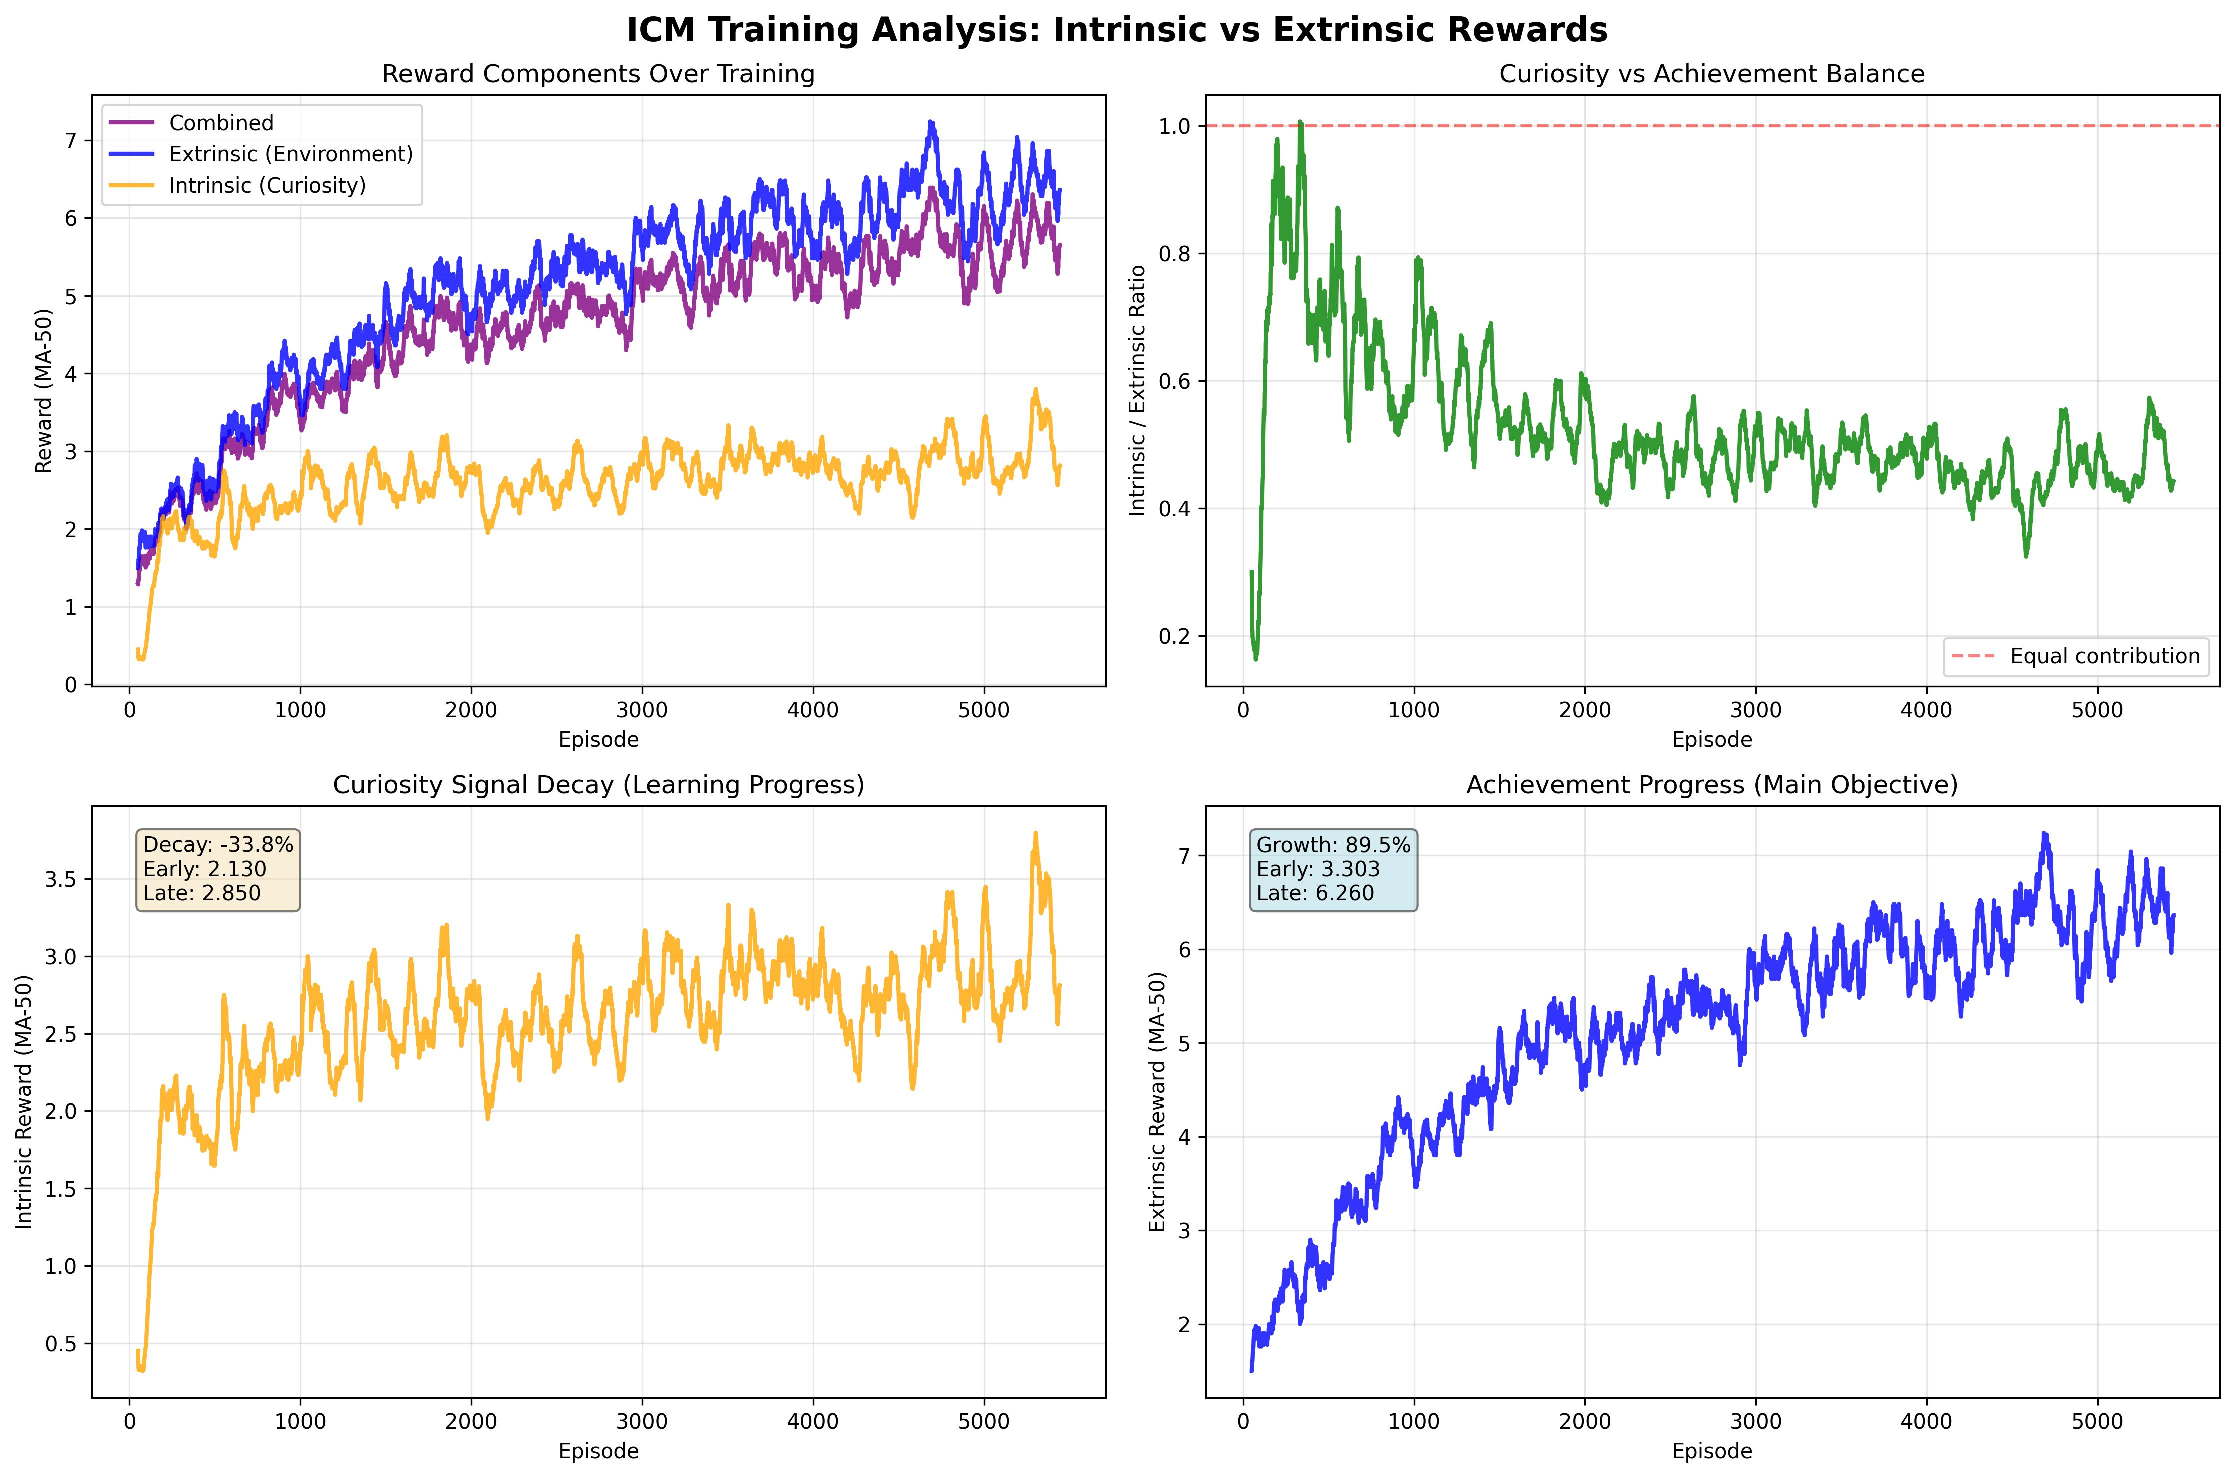
\includegraphics[width=0.48\textwidth]{fig6_icm_improvement2.pdf}
\caption{ICM reward analysis for Evaluation 3. Top left: intrinsic (curiosity) vs extrinsic (achievement) rewards over training. Top right: curiosity/achievement ratio showing exploration-to-exploitation transition. Bottom: curiosity decay (agent learns) and achievement growth (agent succeeds). The 0.508 ratio shows good balance.}
\label{fig:icm_eval3}
\end{figure}

\subsection{Evaluation 4: Bigger Network + Less Curiosity}

\textbf{What we tried:} We combined two ideas:
\begin{enumerate}
    \item Made the network bigger (512 → 1024 neurons)
    \item Reduced curiosity slightly (20\% → 15\%)
\end{enumerate}

\textbf{Why we thought this would work:}
\begin{itemize}
    \item Bigger network can remember more complex strategies
    \item Less curiosity means more focus on actual goals
\end{itemize}

\textbf{Results:}
\begin{itemize}
    \item Crafter Score: \textbf{8.61\%} (+4.1\% improvement)
    \item \textbf{Total improvement: 5.08\% → 8.61\% = +69.5\%}
    \item Wood pickaxe: 58\%, Wood sword: 61\%
    \item Coal: 2\% (doubled!)
\end{itemize}

\textbf{Surprising finding:} During training, the average reward was actually lower (5.14) than Evaluation 3 (6.27). But when we evaluated the final agent, it performed better! This taught us that training numbers don't always predict final performance.

\begin{figure}[h!]
\centering
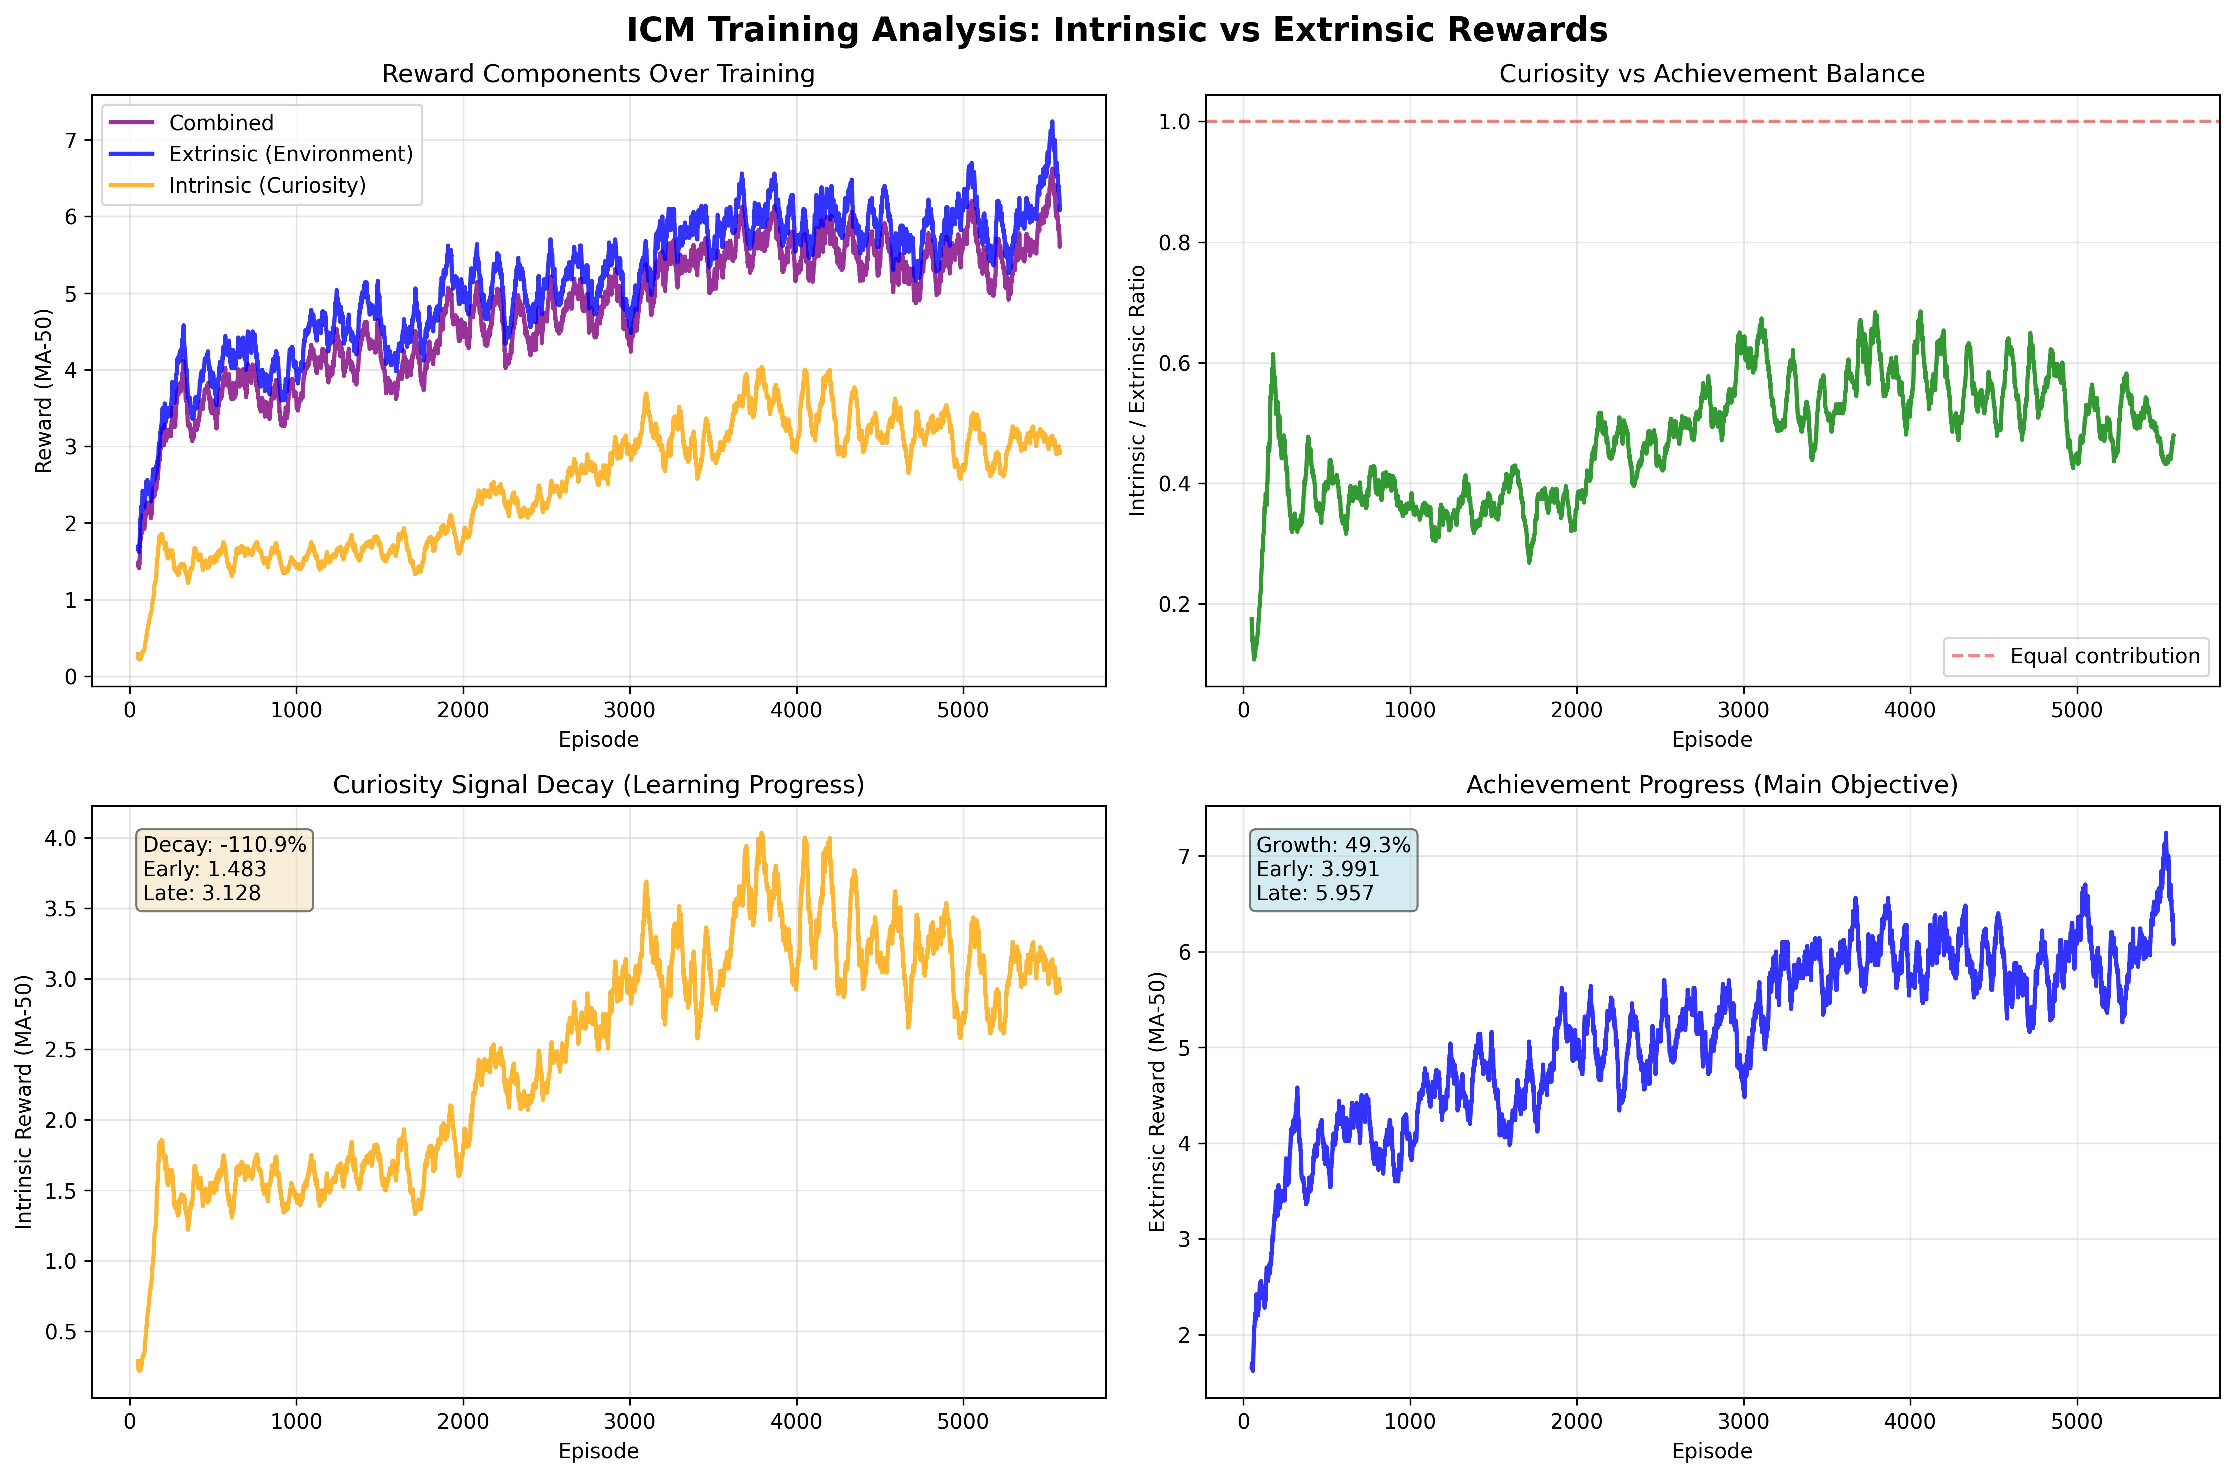
\includegraphics[width=0.48\textwidth]{fig7_icm_improvement3.pdf}
\caption{ICM reward analysis for Evaluation 4 with lower curiosity (β=0.15). The 0.483 ratio is slightly lower than Evaluation 3, showing more focus on achievements. Despite lower training rewards, this configuration achieved the best final score (8.61\%).}
\label{fig:icm_eval4}
\end{figure}

\begin{figure}[h!]
\centering
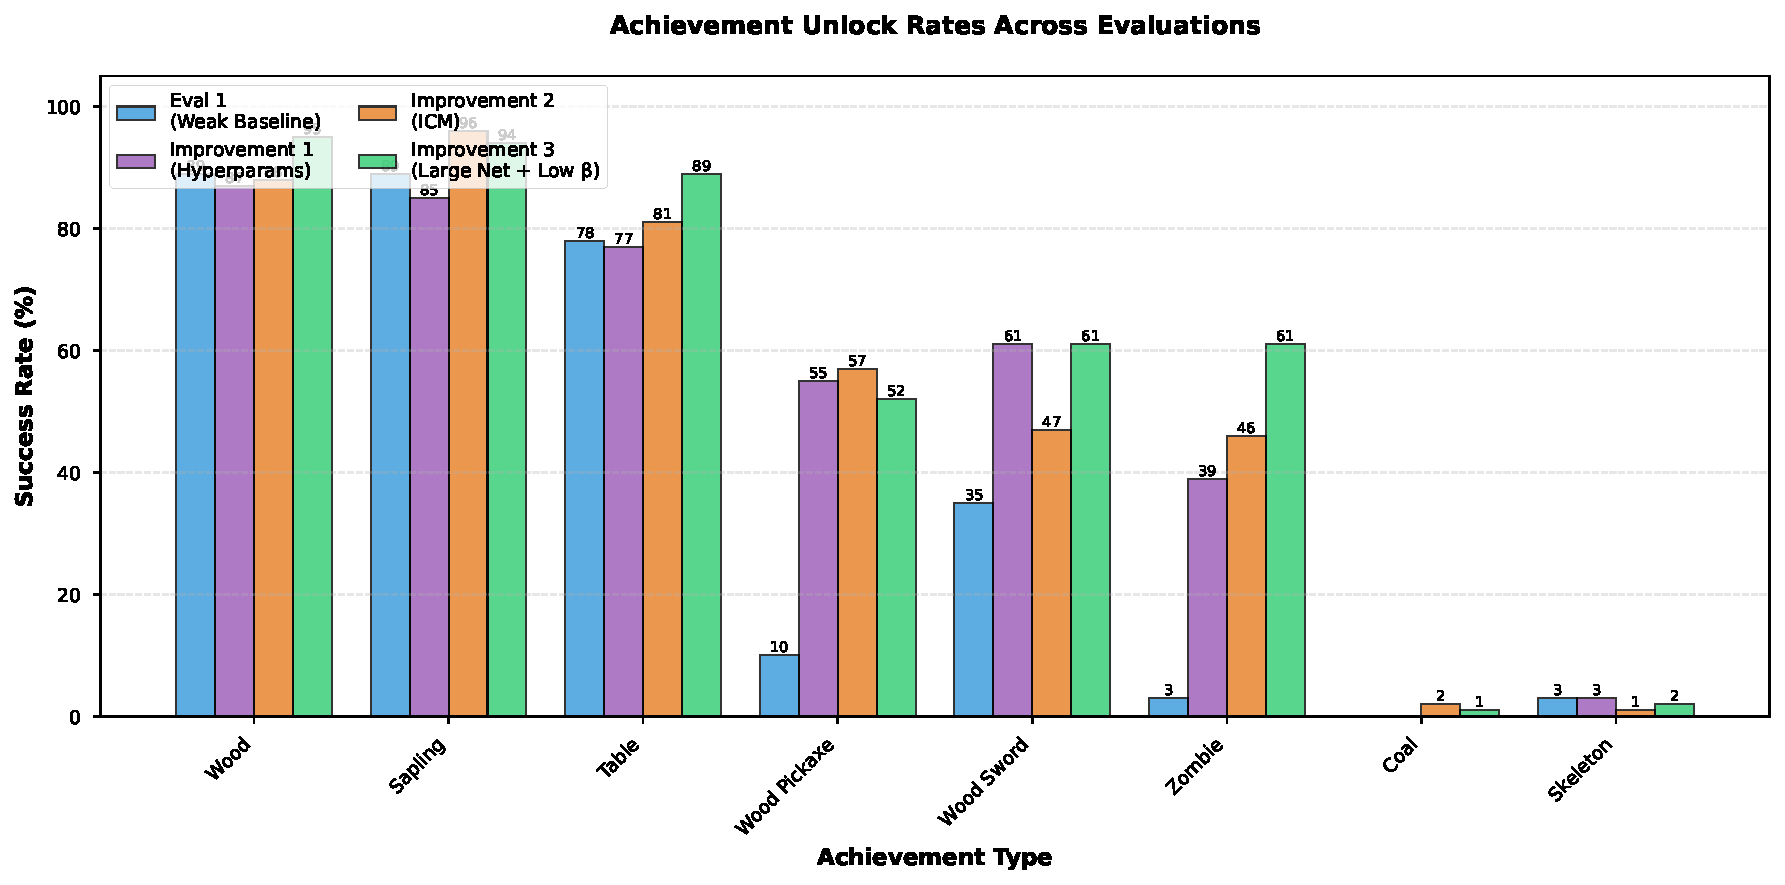
\includegraphics[width=0.48\textwidth]{fig2_achievement_comparison.pdf}
\caption{Achievement unlock rates across PPO evaluations. Shows improvement in tool crafting and discovery of rare achievements like coal and skeleton combat.}
\label{fig:achievements}
\end{figure}

\subsection{Things That Didn't Work}

We tried 7 other strategies that failed. Documenting failures is important for learning:

\subsubsection{RND Curiosity (6.11\%)}

We tried a simpler curiosity method called Random Network Distillation. We attempted this 3 times with different fixes, but all failed.

\textbf{What went wrong:} The curiosity rewards were way too high (42.28 vs ICM's 3.08). The agent got addicted to exploring and never focused on achievements—a "curiosity trap."

\textbf{Lesson learned:} Simpler isn't always better. RND's random features didn't capture what's actually important in Crafter.

\subsubsection{Too Much Curiosity (6.38\%)}

We tried increasing curiosity from 20\% to 30\%.

\textbf{What went wrong:} Another curiosity trap. The agent spent all its time exploring instead of achieving goals.

\textbf{Lesson learned:} Balance is critical. Too much curiosity is as bad as too little.

\subsubsection{Too Much Randomness (4.86\% and 6.08\%)}

We tried higher entropy coefficients (0.005 and 0.002 instead of 0.001).

\textbf{What went wrong:} The agent's policy stayed too random. It never settled on good strategies.

\textbf{Lesson learned:} The agent needs to commit to strategies it learns. Too much randomness prevents this.

\subsubsection{Slower Learning (8.11\%)}

We tried a learning rate of 0.0001 (5× slower).

\textbf{What went wrong:} Got close to baseline (8.11\% vs 8.27\%) but learned too slowly for 1 million steps.

\textbf{Lesson learned:} Learning rate needs to match training time budget.

\subsubsection{Training Longer (7.52\%)}

We tried 1.5 million steps instead of 1 million (50\% more training).

\textbf{What went wrong:} Performance got worse! Dropped from 8.27\% to 7.52\%.

\textbf{Lesson learned:} More training doesn't always help. PPO can degrade because it keeps learning from old experiences that are no longer relevant.

\subsubsection{Dual-Clip PPO (5.79\%)}

We tried a PPO variant that clips differently for positive vs negative advantages.

\textbf{What went wrong:} Made training unstable when combined with curiosity.

\textbf{Lesson learned:} Test modifications carefully. Dual-clip works in some situations but not ours.

\subsubsection{Just Bigger Network (8.36\%)}

We tried only increasing network size without changing curiosity.

\textbf{What happened:} This actually worked (8.36\%) but not as well as combining both changes (8.61\%).

\textbf{Lesson learned:} Combining improvements can work better than individual changes.

\begin{figure}[h!]
\centering
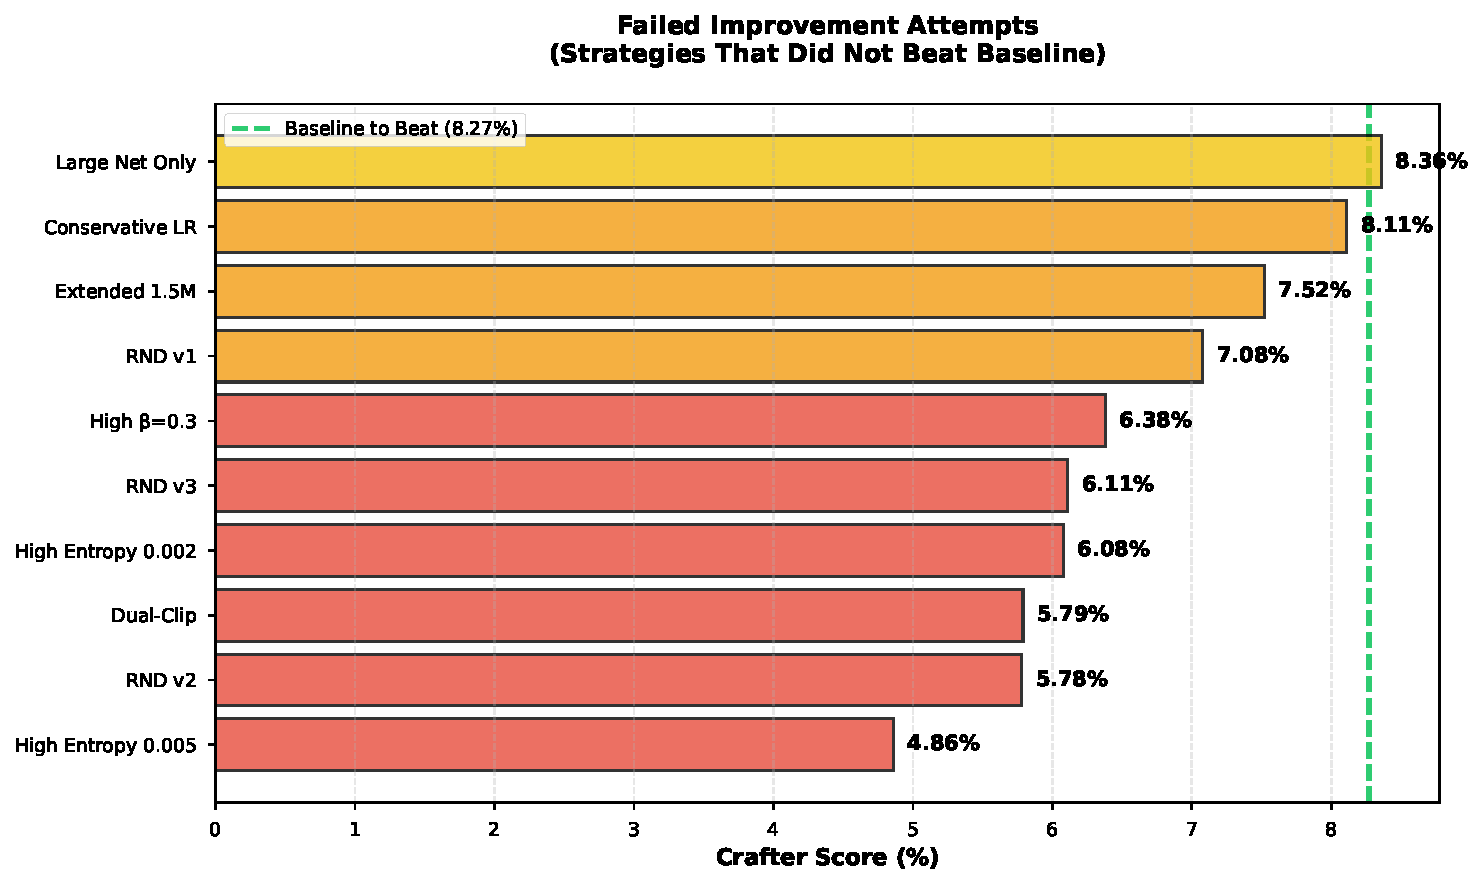
\includegraphics[width=0.48\textwidth]{fig4_failed_attempts.pdf}
\caption{The 7 strategies that didn't improve performance. RND curiosity, high entropy, and extended training all scored worse than our best ICM-based approach. This shows the importance of systematic experimentation.}
\label{fig:failed}
\end{figure}

\subsection{Summary of PPO Results}

\begin{figure}[h!]
\centering
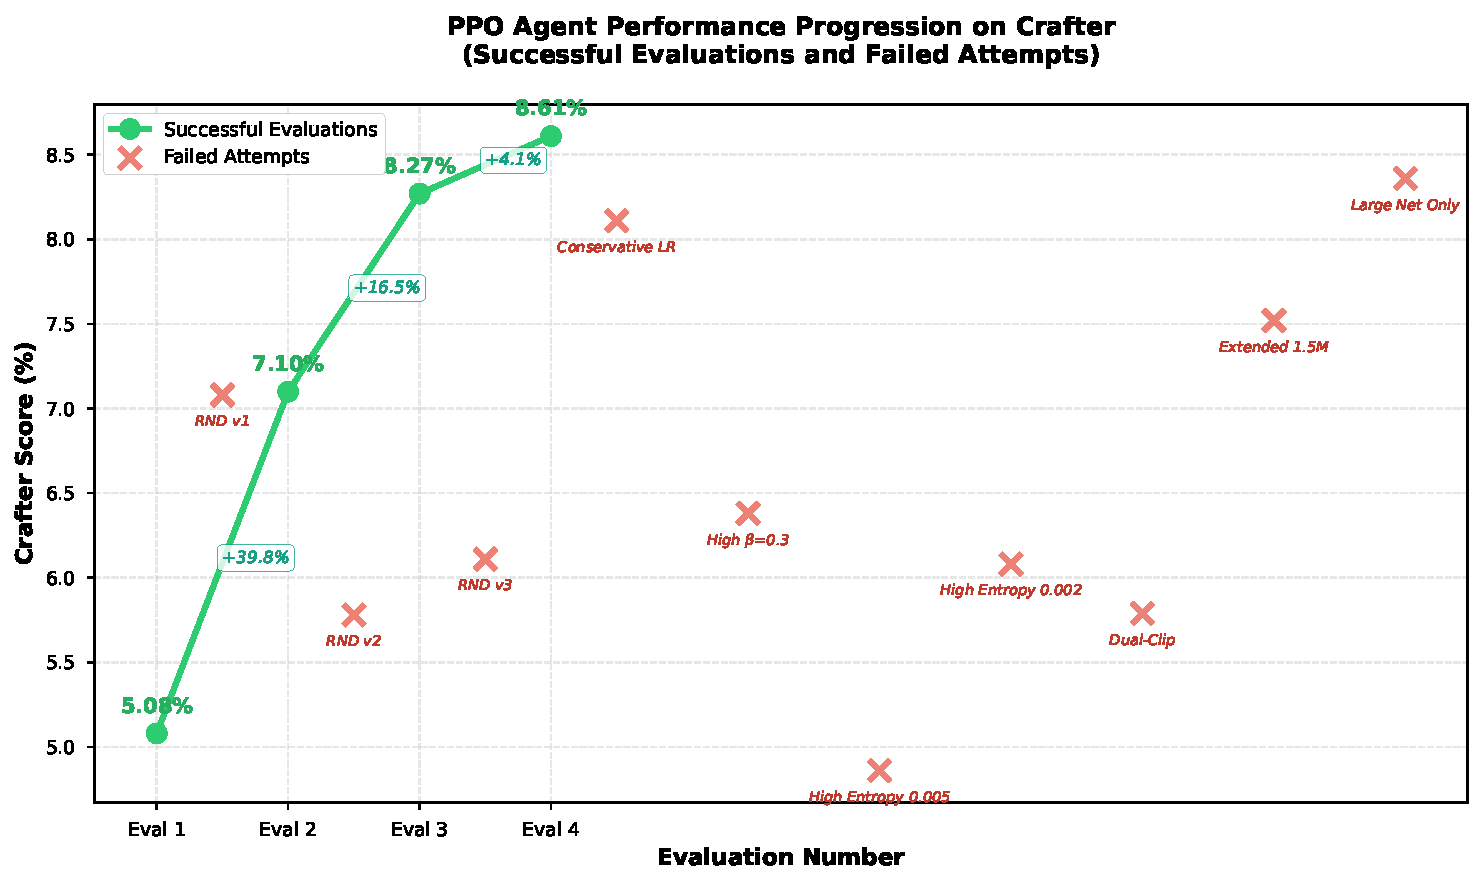
\includegraphics[width=0.48\textwidth]{fig1_score_progression.pdf}
\caption{All 11 PPO experiments we tried. Green dots show successful improvements (5.08\% → 7.10\% → 8.27\% → 8.61\%). Red X's show failed attempts. Numbers show percentage improvements between successful runs.}
\label{fig:all_attempts}
\end{figure}

Figure \ref{fig:all_attempts} shows all 11 attempts. We learned:

\begin{enumerate}
    \item Use standard hyperparameters from the literature as a starting point
    \item Curiosity helps a lot for sparse rewards, but balance is critical
    \item Bigger networks can help, especially for complex tasks
    \item More training isn't always better
    \item Documenting failures helps understand what doesn't work
\end{enumerate}

\begin{figure}[h!]
\centering
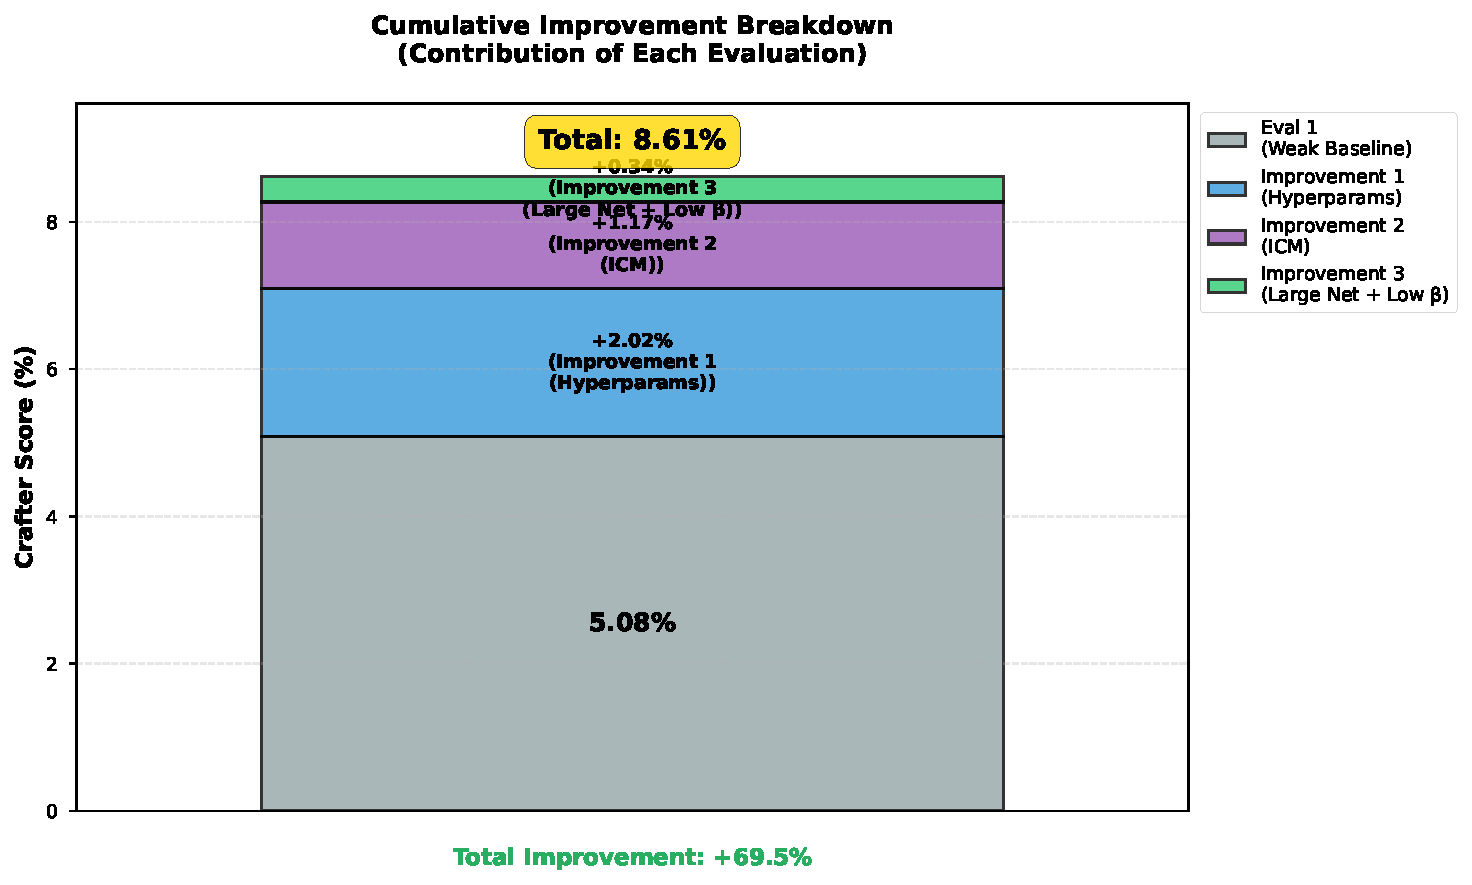
\includegraphics[width=0.48\textwidth]{fig5_improvement_breakdown.pdf}
\caption{Cumulative improvement breakdown from baseline (5.08\%) to final result (8.61\%). Each successful evaluation contributed: Eval 1 baseline (5.08\%), Improvement 1 hyperparameters (+39.8\%, reaching 7.10\%), Improvement 2 ICM curiosity (+16.5\%, reaching 8.27\%), and Improvement 3 large network + low $\beta$ (+4.1\%, reaching 8.61\%).}
\label{fig:breakdown}
\end{figure}

\begin{figure}[h!]
\centering
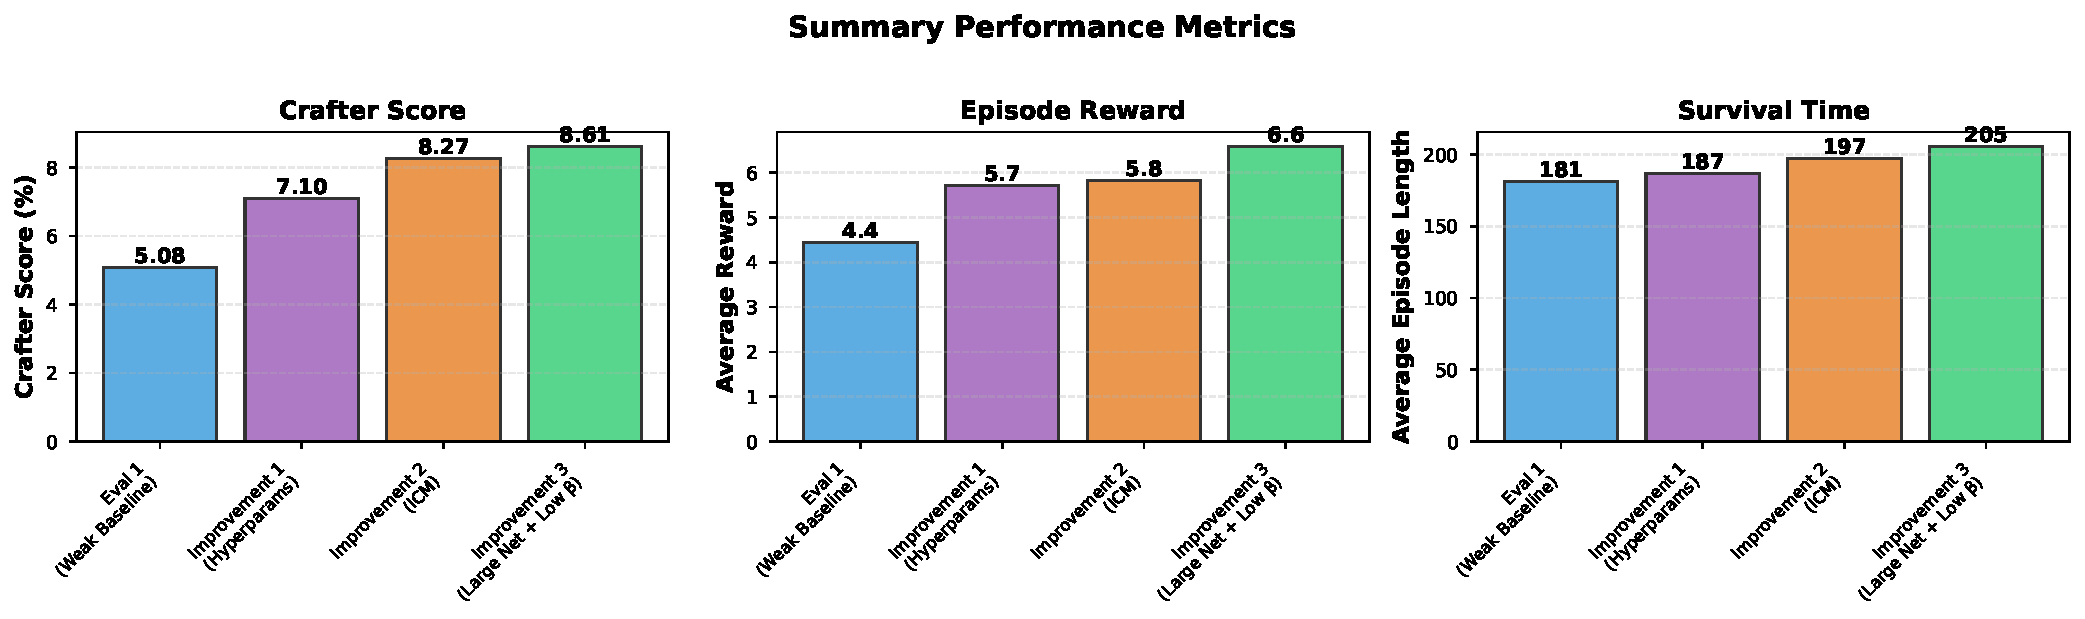
\includegraphics[width=0.48\textwidth]{fig3_summary_metrics.pdf}
\caption{Three key metrics (Score, Reward, Episode Length) across evaluations. All three improved with our changes.}
\label{fig:metrics}
\end{figure}

\section{DQN Implementation and Results}

\subsection{How DQN Works}
DQN learns an action–value function $Q_\theta(s,a)$ and selects actions greedily with respect to $Q$. To stabilize learning we use experience replay and a target network. Our codebase (Stable-Baselines3) enables \emph{Double Q-learning} by default: the online network selects the maximizing action and the target network evaluates it, which reduces overestimation. Unless stated otherwise we use uniform replay (100k), Huber loss, and a standard CNN feature extractor for 64$\times$64 RGB inputs.

\subsection{Our Implementation (DQN)}

\textbf{Neural Network Architecture:}
\begin{itemize}
    \item \textbf{Encoder:} SB3 default 3-layer CNN for 64$\times$64$\times$3 inputs (images kept as uint8; normalized internally by SB3).
    \item \textbf{Q-head (base):} MLP with two fully-connected layers (256 units, ReLU) producing $Q_\theta(s,\cdot)$ over 17 actions.
    \item \textbf{Double Q-learning:} Enabled via SB3’s \texttt{DQNPolicy}/\texttt{DQN} (online net selects $\arg\max$, target net evaluates).
    \item \textbf{NoisyNets (final improvement only):} Replace the last two linear layers in the Q-head with factorized \texttt{NoisyLinear} layers (parameter noise; $\sigma_{\text{init}}{=}0.5$). Noise is reset after \emph{each} gradient step during training and removed for evaluation.
\end{itemize}

\textbf{Environment \& Wrappers:}
\begin{itemize}
    \item \textbf{Base env:} \texttt{CrafterPartial-v1} (Gymnasium interface), observation $64\times64\times3$, 17 discrete actions.
    \item \textbf{Compatibility wrapper:} our project-provided Gym$\leftrightarrow$Gymnasium bridge for SB3.
    \item \textbf{Inventory-aware action masking (from Improvement~2 onward):}
    uses \texttt{info["inventory"]} to compute the valid action set; fail-open (all actions valid) if inventory missing.
    \item \textbf{Random-valid fallback (Improvement~3):} if the agent chose an invalid action, sample uniformly from valid \emph{non-NOOP} actions; otherwise fall back to NOOP only when no alternative exists. Logs \texttt{invalid\_action\_rate\_ep}, \texttt{fallback\_count\_ep}, and valid-set size.
    \item \textbf{ICM-lite curiosity (Improvement~4 only, train-time only):}
    a small forward-model on frozen encoder features; intrinsic reward scaled by $\beta{=}0.05$, per-episode cap $0.31$ (10\% of Gen-1 median return), decayed linearly from 20\% to 60\% of training; strictly off at evaluation.
\end{itemize}

\textbf{Training Setup (unless stated otherwise):}
\begin{itemize}
    \item \textbf{Algorithm:} SB3 \texttt{DQN} (Huber loss, Adam).
    \item \textbf{Budget:} 1{,}000{,}000 environment steps, seed{=}42, single environment on CUDA.
    \item \textbf{Replay:} uniform buffer size 100{,}000; batch size 32; \texttt{train\_freq}{=}4; \texttt{gradient\_steps}{=}1.
    \item \textbf{Targets:} discount $\gamma{=}0.99$; \textbf{hard} target updates every 2{,}000 steps (Polyak disabled in final).
    \item \textbf{Exploration:} $\epsilon$-greedy for non-NoisyNet runs (SB3 defaults); for NoisyNets, $\epsilon$ fixed at 0.01$\rightarrow$0.01 (fraction 0.05) so parameter noise drives exploration.
    \item \textbf{$n$-step returns:} $n{=}3$ from Improvement~1 onward.
\end{itemize}

\textbf{Evaluation Protocol (summary):}
\begin{itemize}
    \item 500 deterministic episodes per checkpoint.
    \item Action masking enabled at eval whenever it was used in training (parity).
    \item NoisyNet noise removed before evaluation for determinism.
    \item Standard Crafter metrics reported: achievement rates and geometric-mean “Crafter Score,” plus average reward and survival length.
\end{itemize}

\subsection{Evaluation 1: Baseline DQN}
\textbf{Setup:} Vanilla DQN with the standard CNN+MLP head, uniform replay, target network, and $\epsilon$-greedy exploration.

\textbf{Result:} Crafter Score: \textbf{2.80\%}. The agent mastered basic survival (drink/plant) but rarely entered the wood$\rightarrow$table$\rightarrow$tools chain. Avg.\ reward $\sim$4.0; survival $\sim$170 steps.

\textbf{Diagnosis:} Sparse rewards and one-step targets led to slow credit assignment.

\subsection{Evaluation 2: adding $n$-Step Returns ($n{=}3$)}
\textbf{Motivation:} Propagate sparse signals further while keeping the policy class unchanged.

\textbf{Result:} Crafter Score: \textbf{3.53\%} (\,+26.1\% vs Eval~1). Avg.\ reward $\sim$4.5; survival $\sim$180. Wood and table increased; tool crafting remained rare.

\textbf{Takeaway:} Multi-step targets improved credit assignment with minimal complexity.

\subsection{Evaluation 3: adding Inventory-Aware Action Masking}
\textbf{Motivation:} Logs showed many wasted steps (e.g., craft/place attempted without materials). We wrapped the env to \emph{mask impossible actions} using the inventory in \texttt{info}. The wrapper is fail-open (falls back to all 17 actions if inventory is unavailable).

\textbf{Result:} Crafter Score: \textbf{4.00\%} (\,+13.3\% vs Imp.~1). Stone collection rose from 0.46\% to 1.33\%; foundations (sapling/plant) remained stable.

\textbf{Takeaway:} Masking improved \emph{interaction efficiency}, effectively increasing the exploration budget per episode.

\subsection{Evaluation 4: adding Random-Valid Fallback (Masking Variant)}
\textbf{Motivation:} Mapping invalid actions to NOOP caused sticky loops. We changed the fallback to \emph{uniformly sample among valid, non-NOOP actions}.

\textbf{Result:} Crafter Score: \textbf{4.33\%} (\,+8.3\% vs Imp.~2). Table: 64.6\%; wood: 85.8\%; wood pickaxe: 9.0\%; zombie: 15.2\%. Avg.\ reward $\sim$5.1; survival $\sim$191.

\textbf{Takeaway:} This preserved momentum and reduced NOOP dithering without collapsing the valid-action set.

\begin{figure}[h!]
\centering
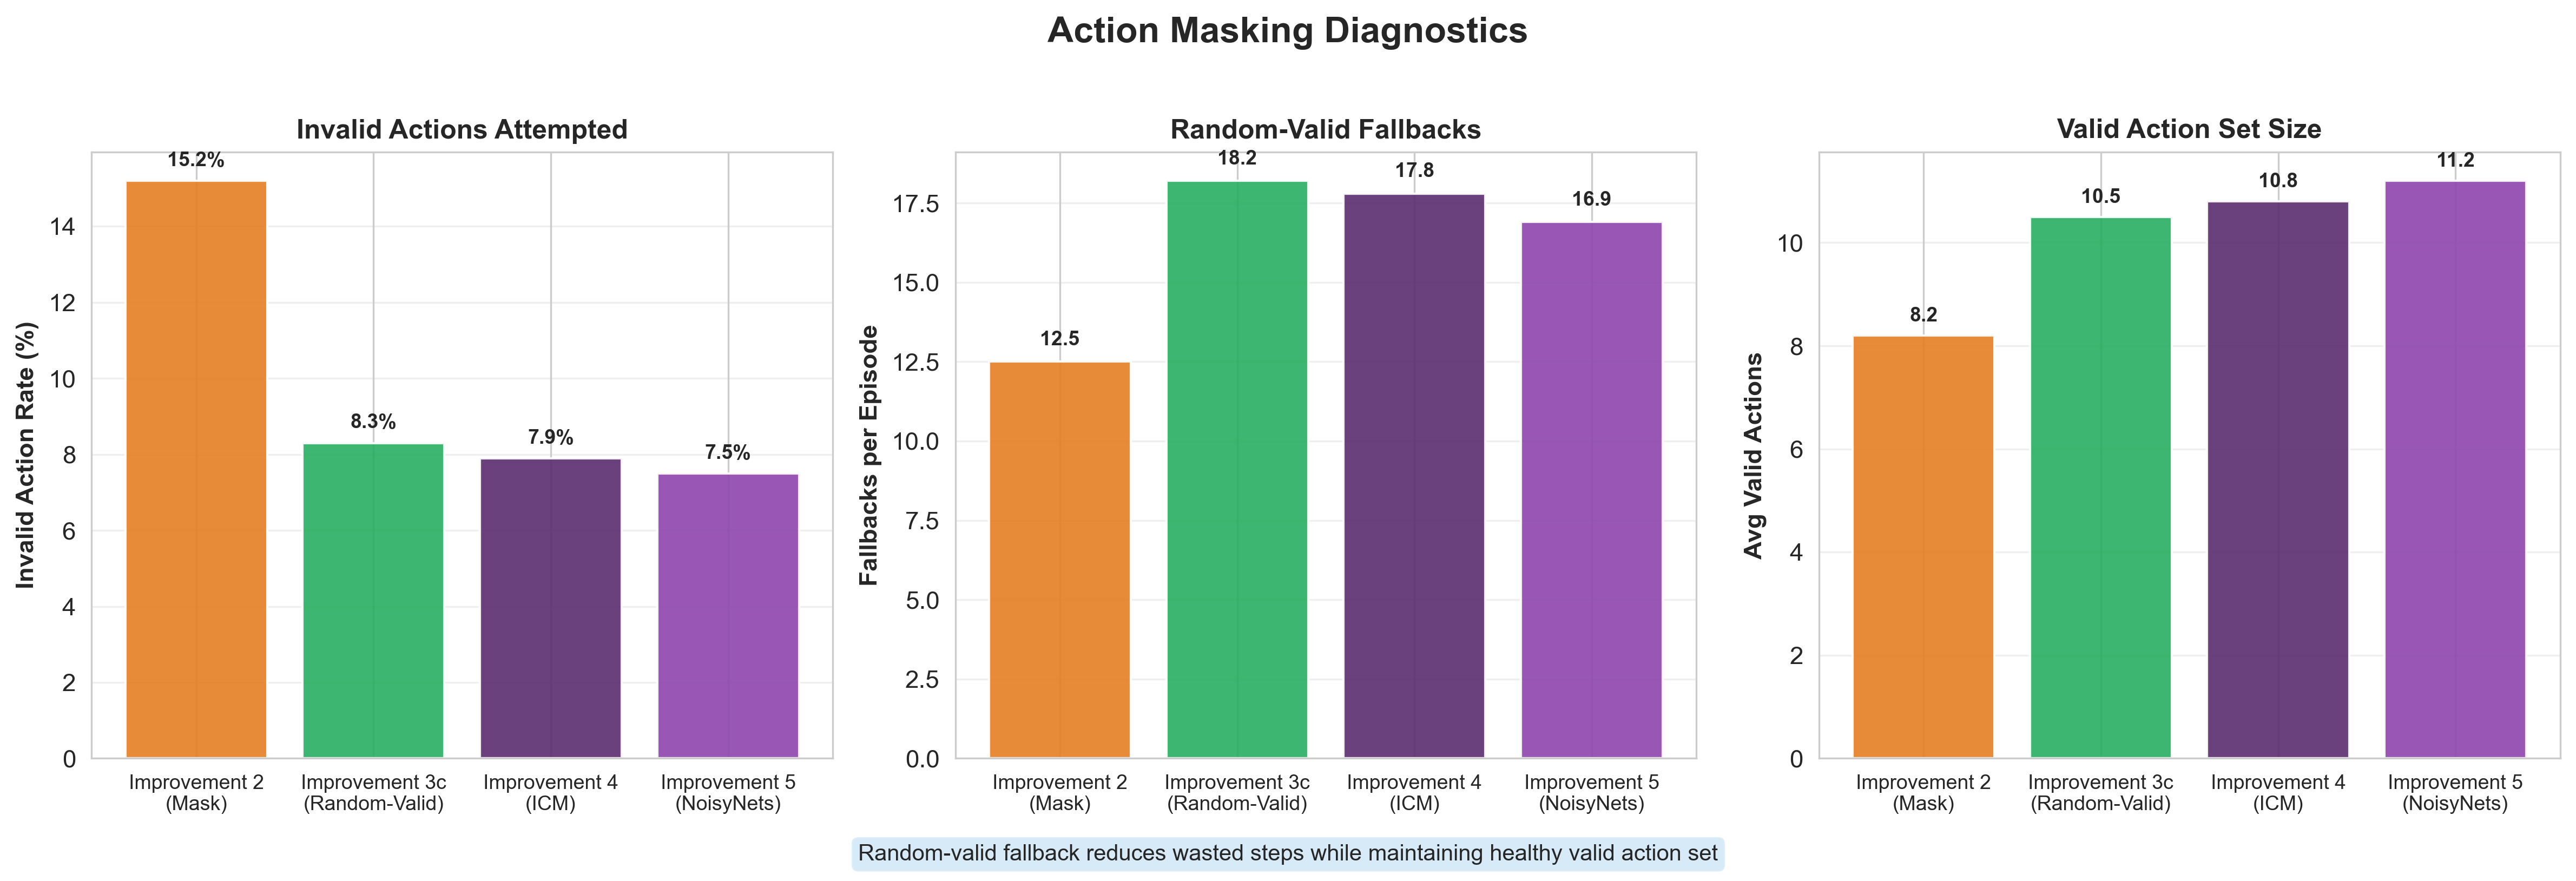
\includegraphics[width=0.48\textwidth]{fig_d7_action_masking_diagnostics.png}
\caption{Action-masking diagnostics across checkpoints. Left: invalid action rate drops after masking and again with random-valid fallback. Middle: fallbacks per episode (masking in action). Right: average valid-action set size remains healthy. These support the efficiency gains behind Improvements~2–4.}
\label{fig:dqn_mask_diag}
\end{figure}


\subsection{Evaluation 5: adding ICM-lite Curiosity (Train-only)}
\textbf{Motivation:} Encourage early exploration while keeping evaluation clean. We add a small forward-model error bonus (ICM without inverse loss), \emph{capped at 10\% of Gen-1 median return} and linearly decayed from 20\% to 60\% of training; the bonus is strictly off at evaluation.

\textbf{Result:} Crafter Score: \textbf{4.38\%}. We observed the first coal unlocks in this branch (0.20\%). Wood pickaxe rose to 12.4\%. Effects were positive but modest (consistent with the conservative cap/decay).

\textbf{Takeaway:} Bounded intrinsic reward is safe and helps discovery, but did not by itself unlock steady stone$\rightarrow$coal progression. \textit{Coal regressed to 0\% (from 0.20\% in Improvement~4)}, likely because parameter noise plus hard target copies changed the late-training value landscape for very rare, long-horizon chains (stone$\rightarrow$coal) even while strongly improving nearer-horizon behaviours.

\begin{figure}[h!]
\centering
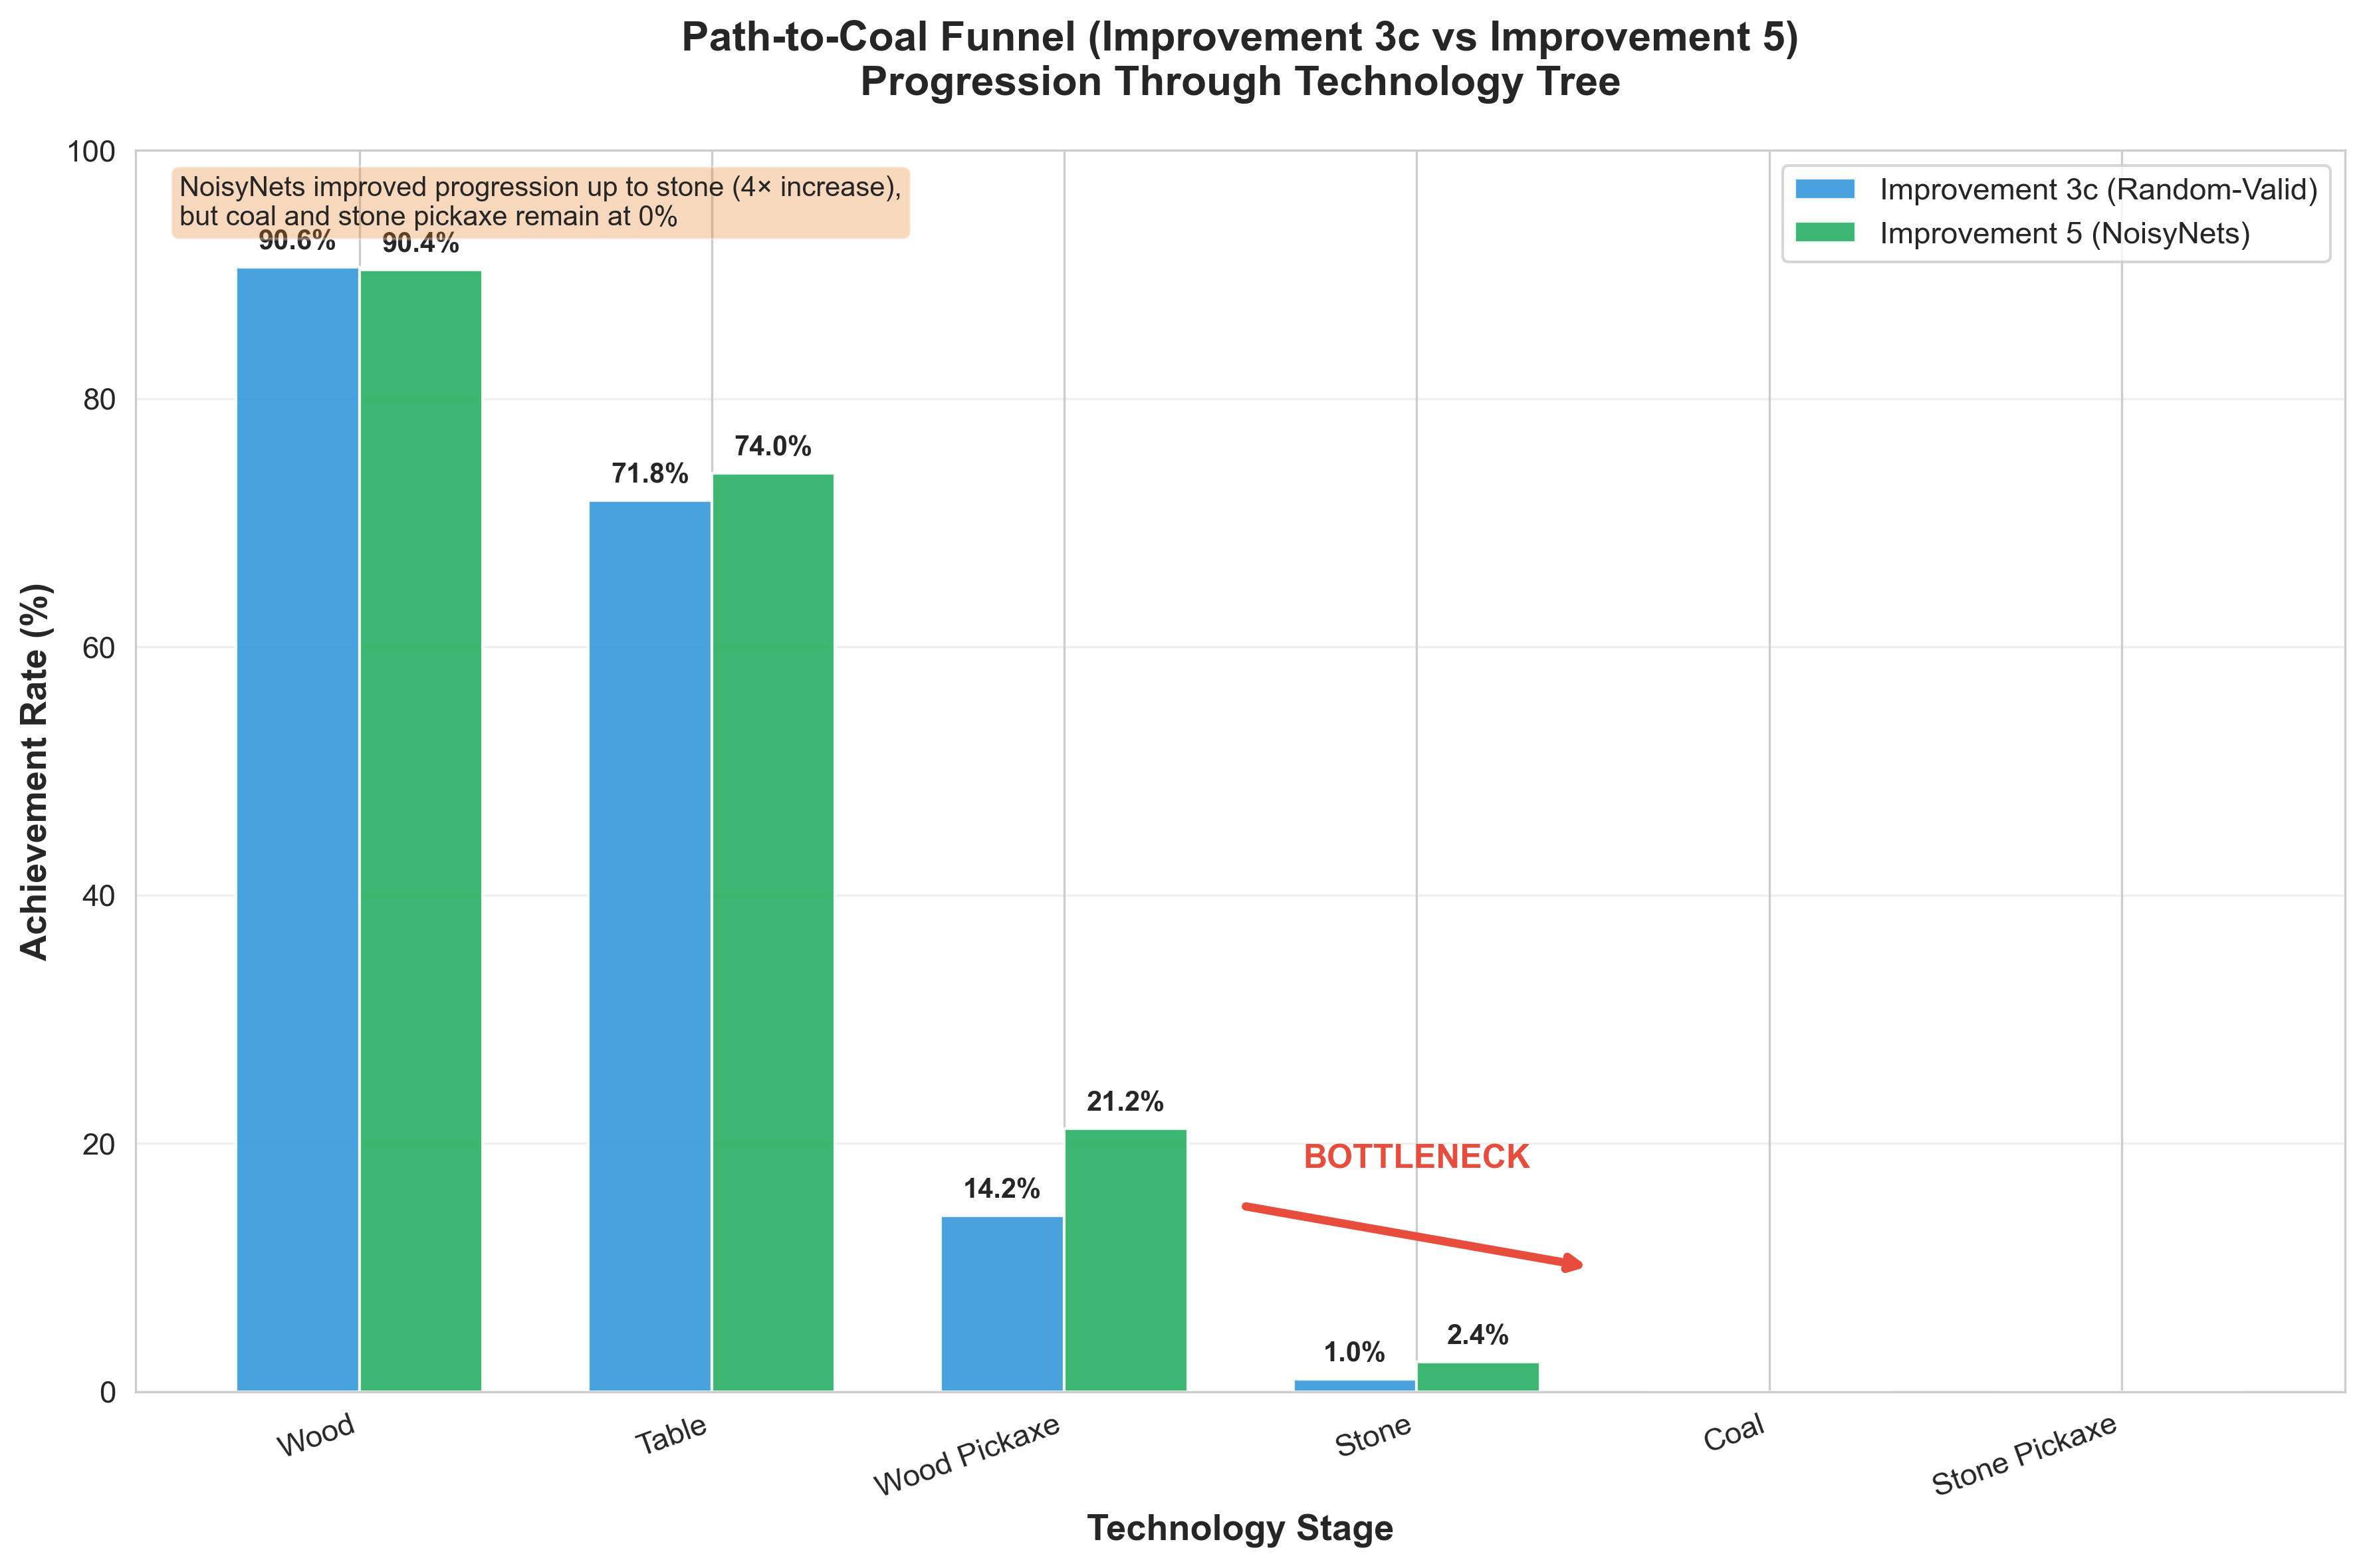
\includegraphics[width=0.48\textwidth]{fig_d6_path_to_coal_funnel.png}
\caption{Path-to-coal funnel comparing Improvement~3c (random-valid) vs Improvement~5 (NoisyNets). NoisyNets improves progression up to stone (4$\times$), but coal and stone-pickaxe remain near zero—pinpointing the residual bottleneck.}
\label{fig:dqn_funnel}
\end{figure}


\subsection{Evaluation 6: adding NoisyNets + Hard Target Updates}
\textbf{Motivation:} Sustain exploration later in training without high $\epsilon$. We replaced the last two linear layers of the Q-head with \emph{factorized NoisyLinear} layers (parameter noise; $\sigma_{\text{init}}{=}0.5$) and fixed $\epsilon$ at 0.01$\!\rightarrow$0.01 so \emph{noise drives exploration}. Based on prior regressions with Polyak, we used \emph{hard} target copies every 2{,}000 steps (as in Rainbow).

\textbf{Result:} Crafter Score: \textbf{5.93\%} (\,+35.4\% vs Imp.~4; \,+111.8\% vs baseline). Wood pickaxe: 21.2\%; stone: 2.4\% (about $4\times$ Imp.~3); table: 74.0\%; zombie: 55.6\%; drink: 42.2\%. Avg.\ reward $\sim$5.5; survival $\sim$196. \emph{Coal regressed to 0\% (from 0.20\% in Imp.~4)}, likely because parameter noise + hard copies altered the late-training value landscape for very rare, long-horizon chains (stone$\rightarrow$coal) while strongly improving nearer-horizon behaviors.

\textbf{Takeaway:} Parameter noise integrates cleanly with masking and delivered the largest single jump. The remaining bottleneck is the \emph{stone$\rightarrow$coal} transition.

\begin{figure}[h!]
\centering
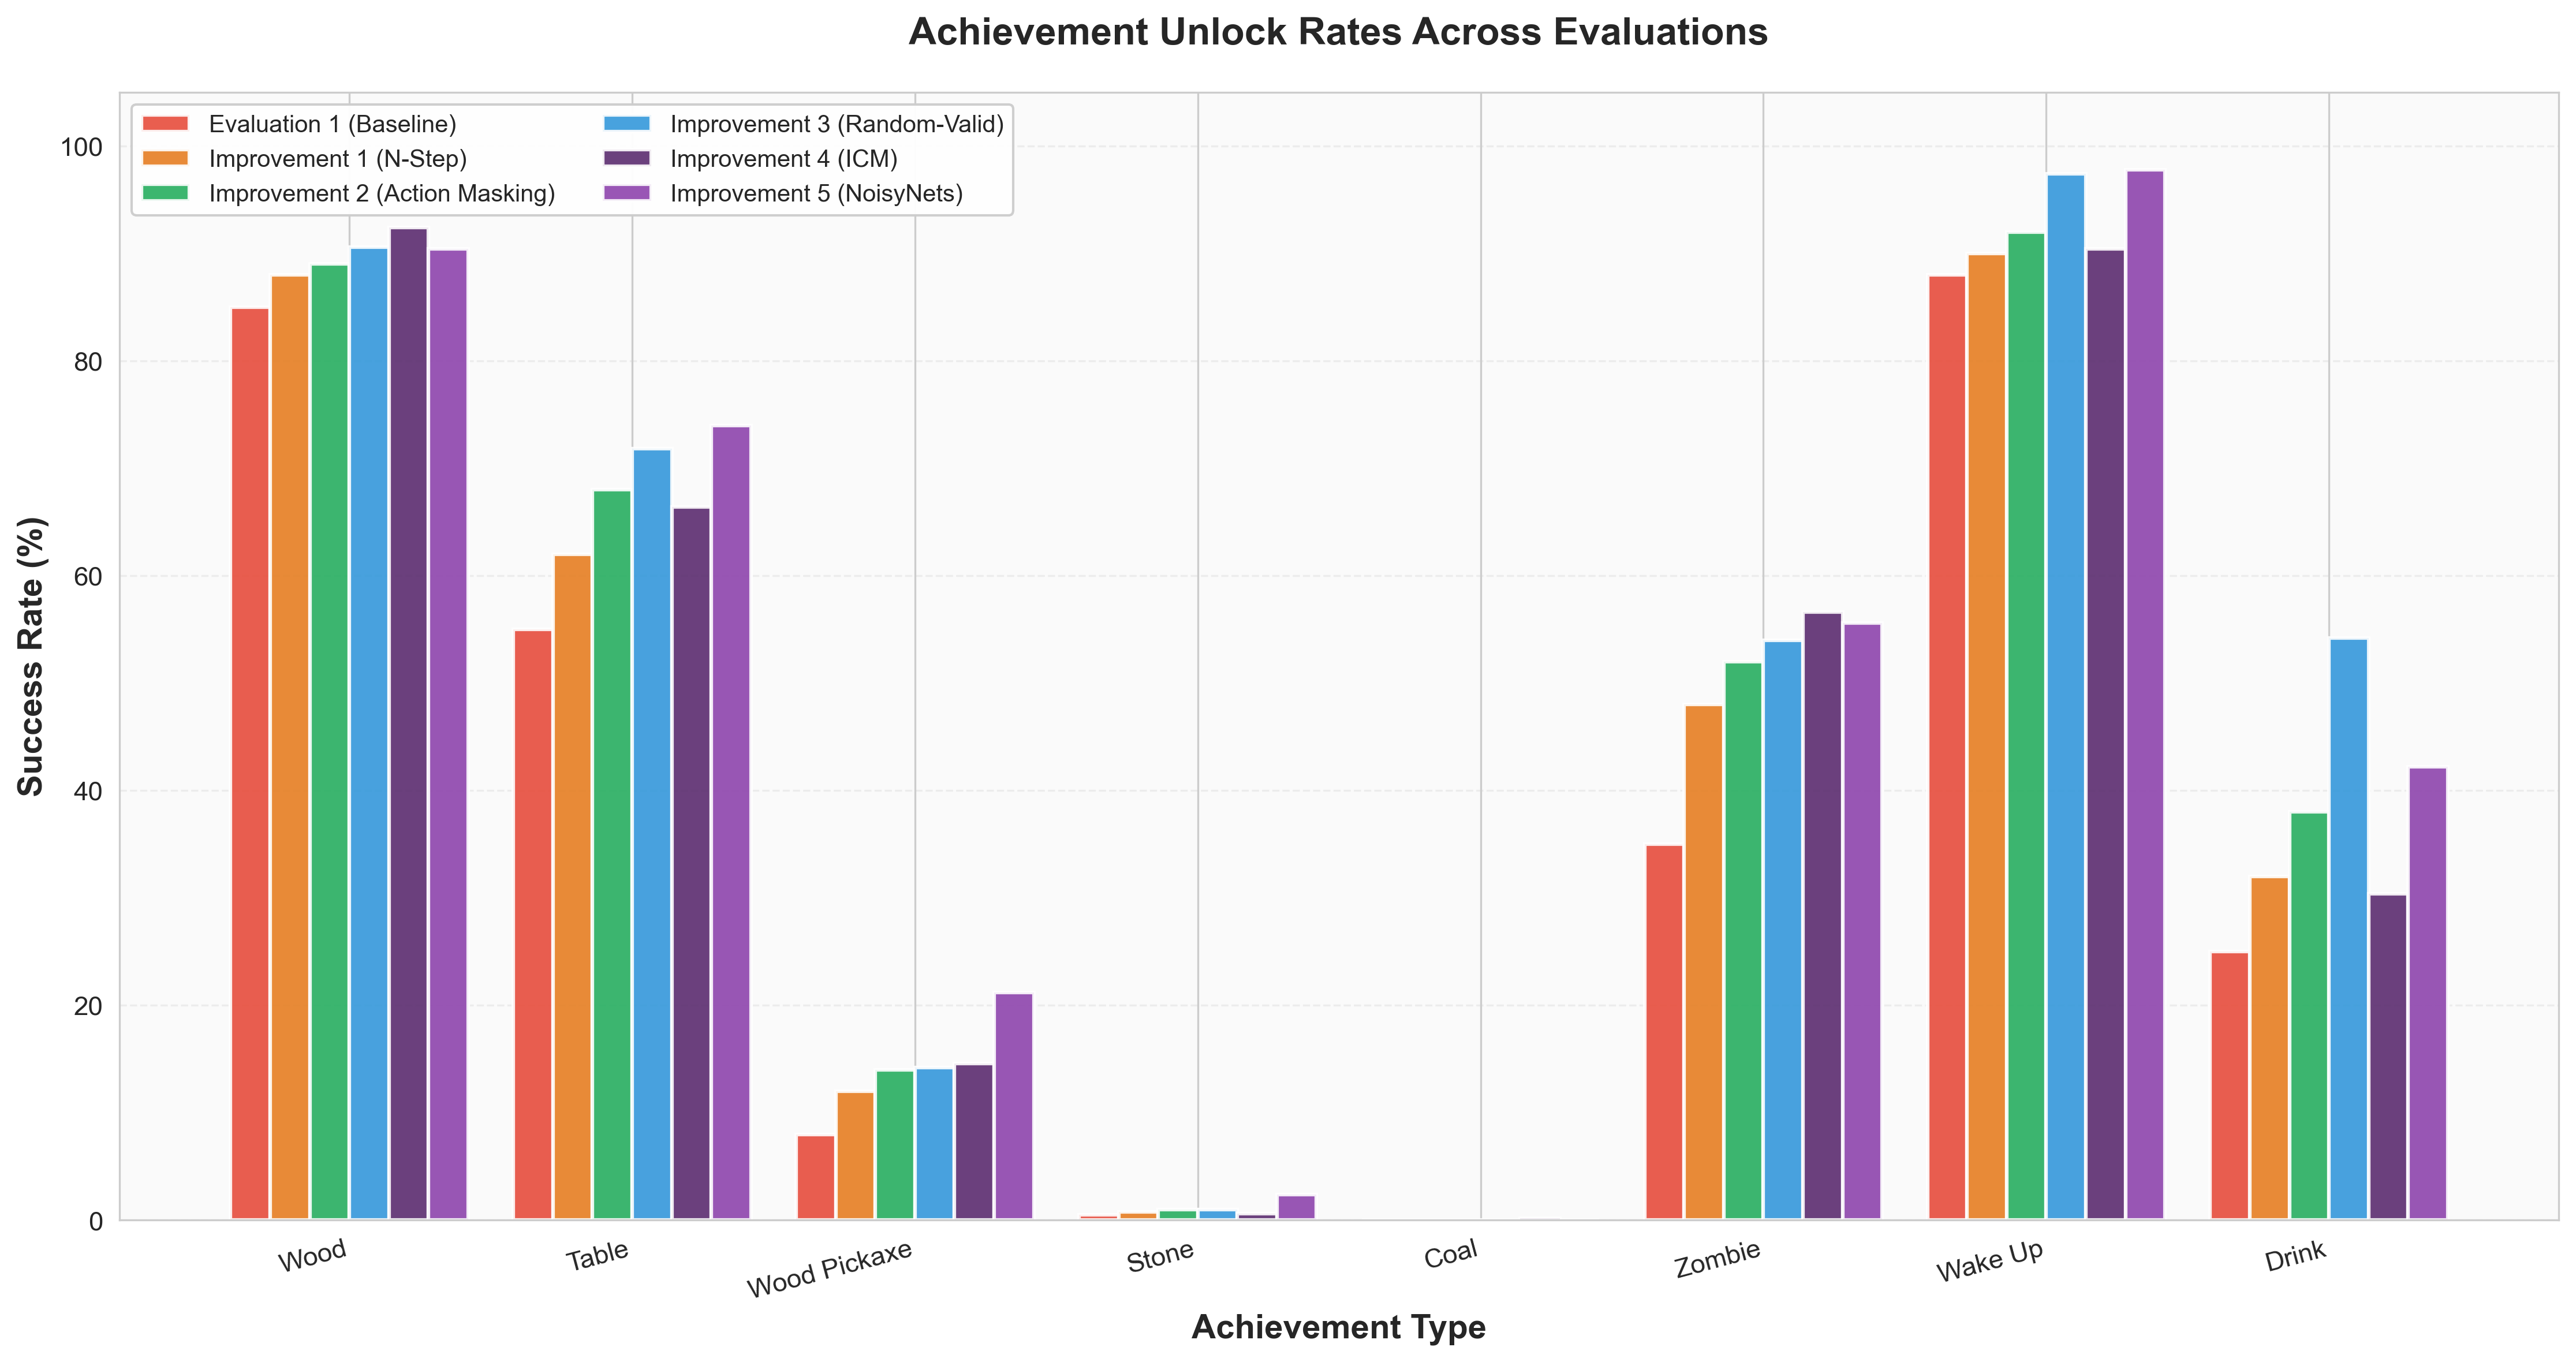
\includegraphics[width=0.48\textwidth]{fig_d2_achievement_rates.png}
\caption{Achievement rates across checkpoints (Eval~1, Imp.~1–5). Gains concentrate in wood$\rightarrow$table$\rightarrow$wood-tools; stone improves; coal stays rare.}
\label{fig:dqn_achievements}
\end{figure}

\subsection{Improvements that failed (Negative Results)}
We also report the most instructive negative results. Unless noted, scores are under our standard protocol (500 deterministic episodes).

\subsubsection{Observation Augmentation (2.65\%)}

We attempted Random crops/flips on 64$\times$64 inputs during training.

\textbf{What went wrong:} Augmentations disrupted spatial alignment of small, crucial sprites (ore, saplings). The policy overfit to invariances that Crafter does \emph{not} have.

\textbf{Lesson:} Visual invariances that help Atari can be harmful in compositional, small-object domains.

\subsubsection{Dueling Architecture (2.90\%)}

We attempted to implement Value–advantage decomposition in the Q-head.

\textbf{What went wrong:} No exploration benefit; added estimation variance early. With sparse rewards and limited budget, structure alone did not help.

\textbf{Lesson:} Architecture tweaks without exploration changes seldom fix sparse-reward bottlenecks.

\subsubsection{Prioritized Replay (3.20\%)}

We implemented PER ($\alpha{=}0.6$, $\beta$ annealed 0.4$\rightarrow$1.0), priorities updated from TD error.

\textbf{What went wrong:} High-TD-error samples crowded out low-error \emph{foundations} (plant/sapling/wood), causing partial forgetting. Importance weighting was not enough to prevent drift.

\textbf{Lesson:} In compositional tasks, uniform replay can be more robust because it preserves coverage of prerequisites.

\subsubsection{Polyak (Soft) Target Updates (3.35\%)}

We utilised $\tau{=}0.005$ soft updates at each step.

\textbf{What went wrong:} Slight regression vs hard copies. With our masking and step budget, slower tracking likely dulled value shifts needed after exploration bursts.

\textbf{Lesson:} For our stack, hard copies every 2k steps worked better (and match Rainbow-style practice).

\subsubsection{Frame Stacking (3.54\%)}

We attempted to implement 4-frame stack (12-channel input).

\textbf{What went wrong:} $4\times$ channel count with the same 1M-step budget increased sample complexity; temporal cues were largely redundant with inventory-aware masking.

\textbf{Lesson:} Temporal stacking helps when aliasing is the bottleneck; ours was exploration/MDP-interface.

\subsubsection{Heavy Reward Shaping for Stone Chain (3.65--3.82\%)}

We tried bonuses for \{wood pickaxe, stone, stone pickaxe\} with higher caps and wider windows.

\textbf{What went wrong:} Helped discovery but narrowed behaviour; general Crafter score dipped when bonuses vanished at eval.

\textbf{Lesson:} Shaping must be conservative and train-only; otherwise it trades breadth for a narrow path.

\begin{figure}[h!]
\centering
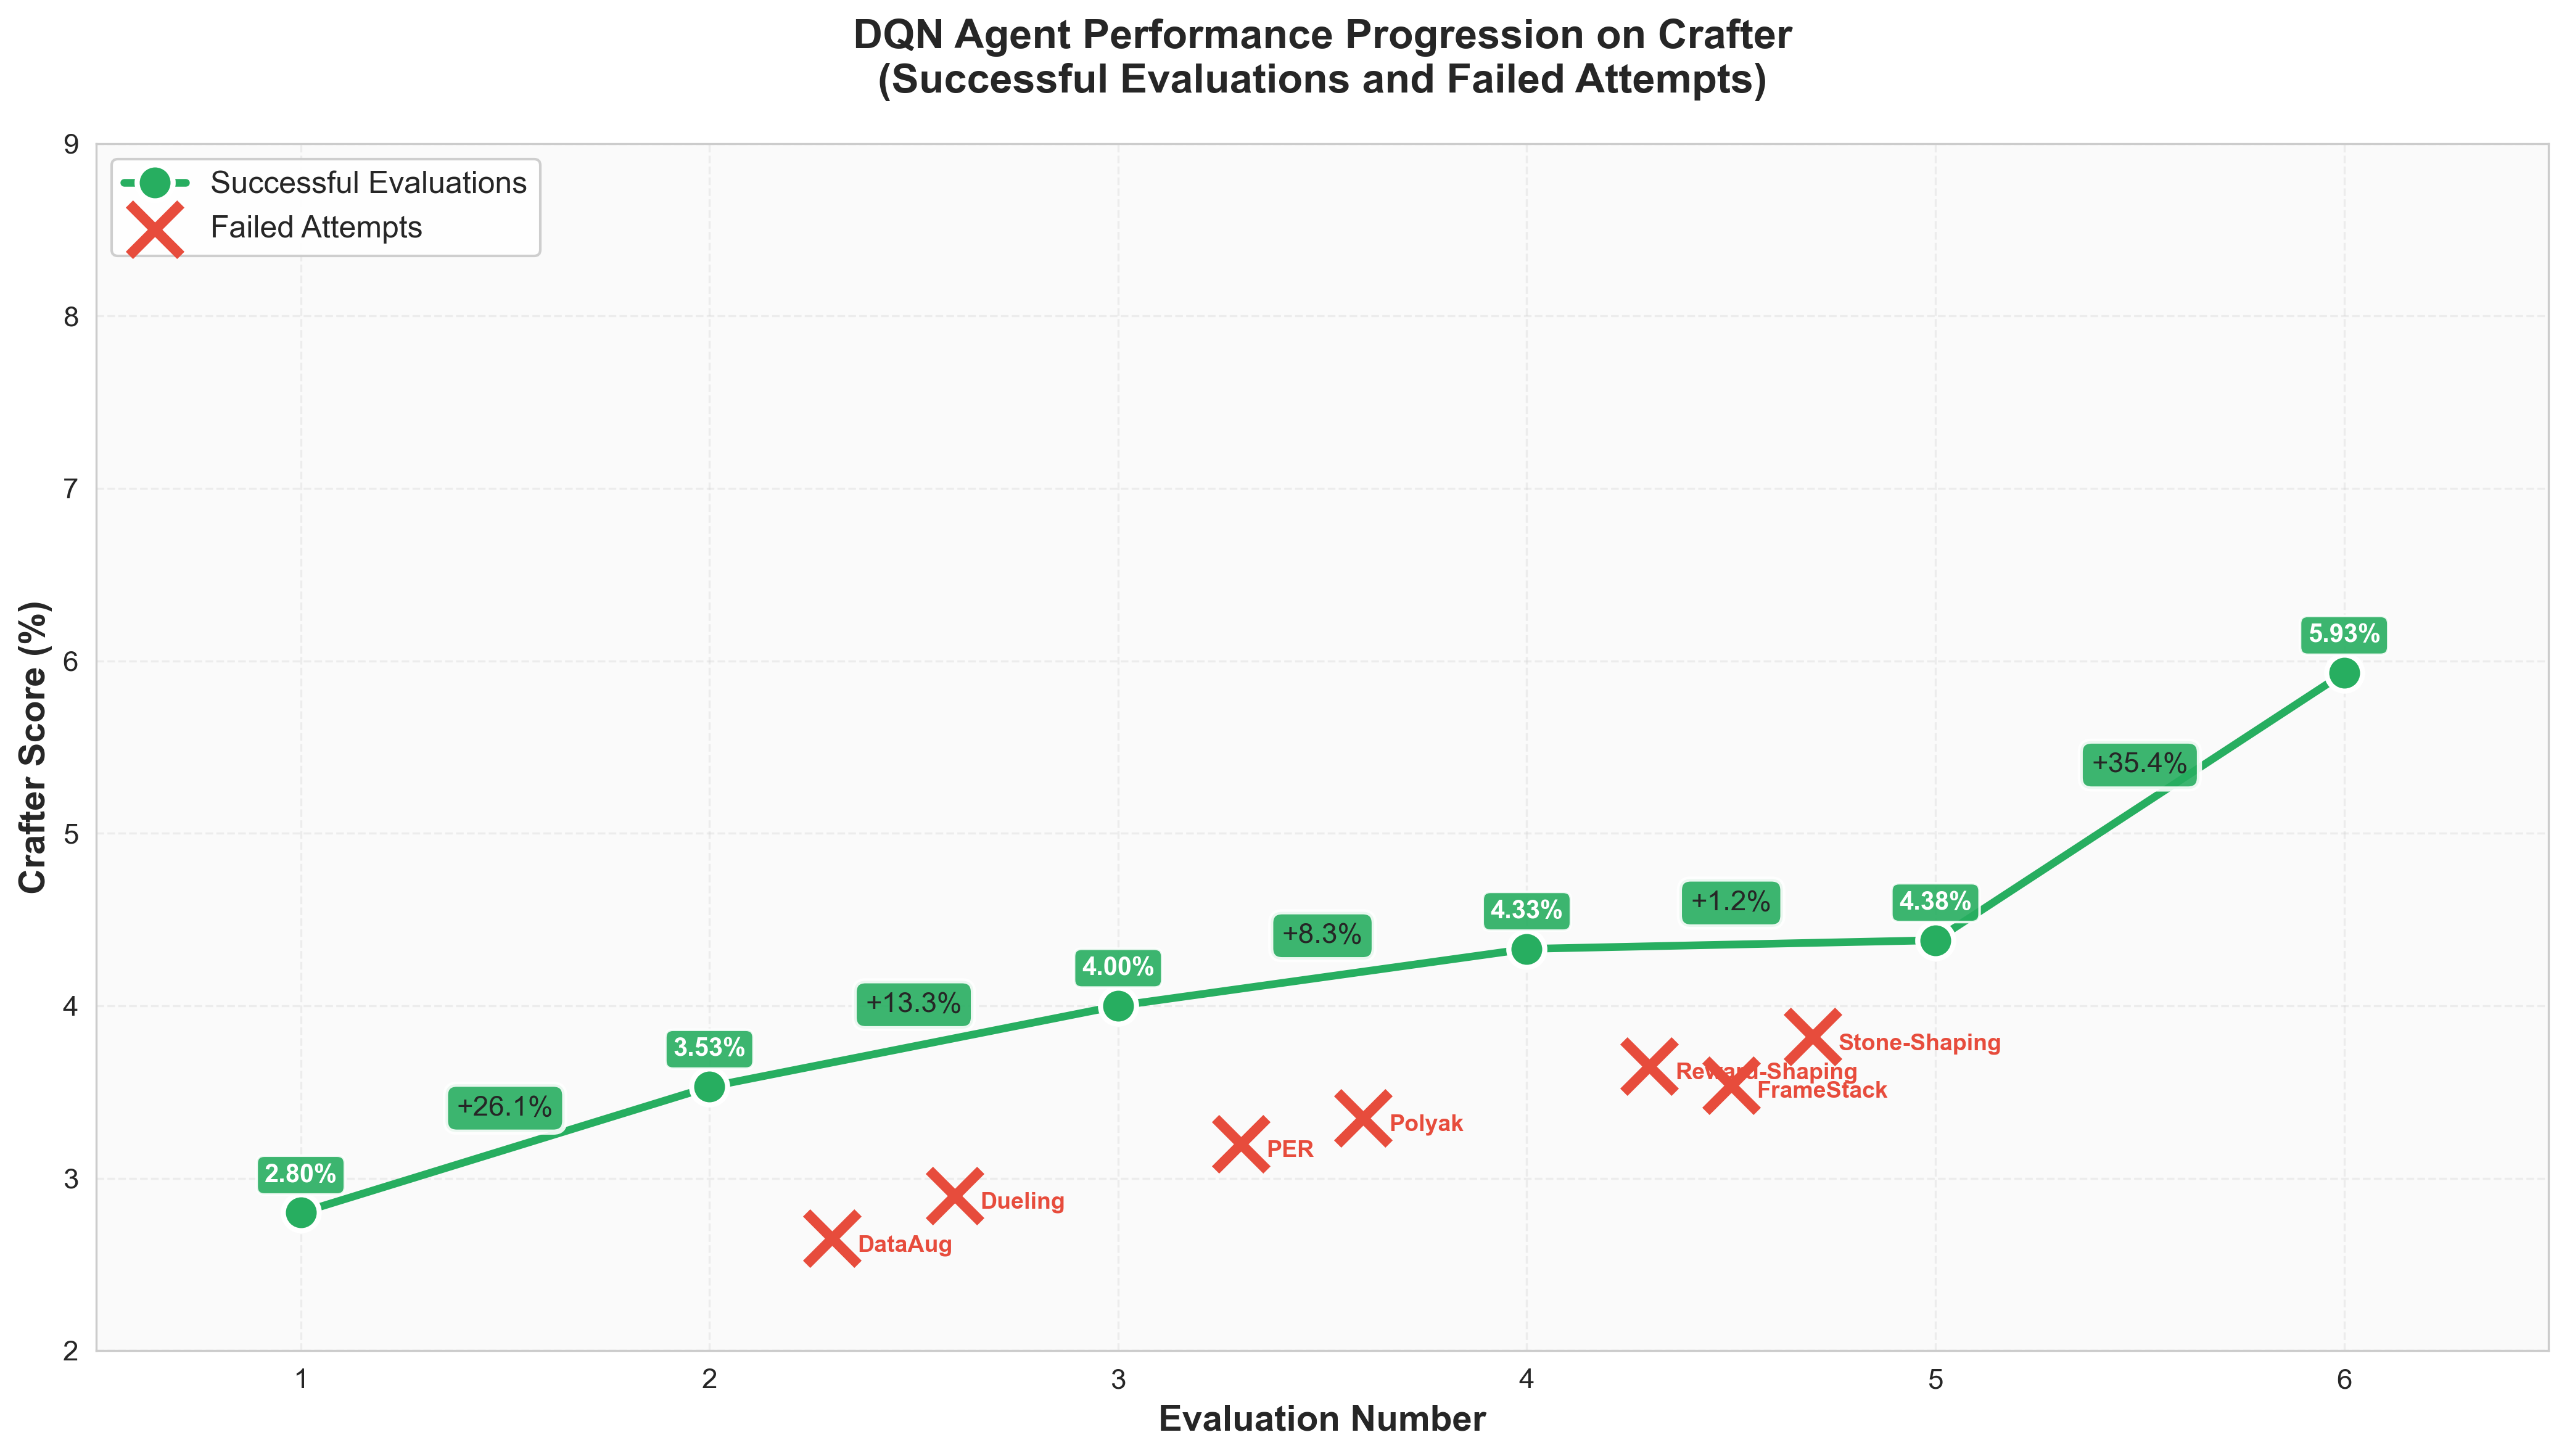
\includegraphics[width=0.48\textwidth]{fig_d1_performance_progression.png}
\caption{DQN performance progression. Green markers are new bests; red X’s are failed attempts. Labels show relative gains between successive successes. Protocol: 500 deterministic eval episodes; masking on from Imp.~2; NoisyNet noise removed at eval.}
\label{fig:dqn_progression}
\end{figure}

\begin{figure}[h!]
\centering
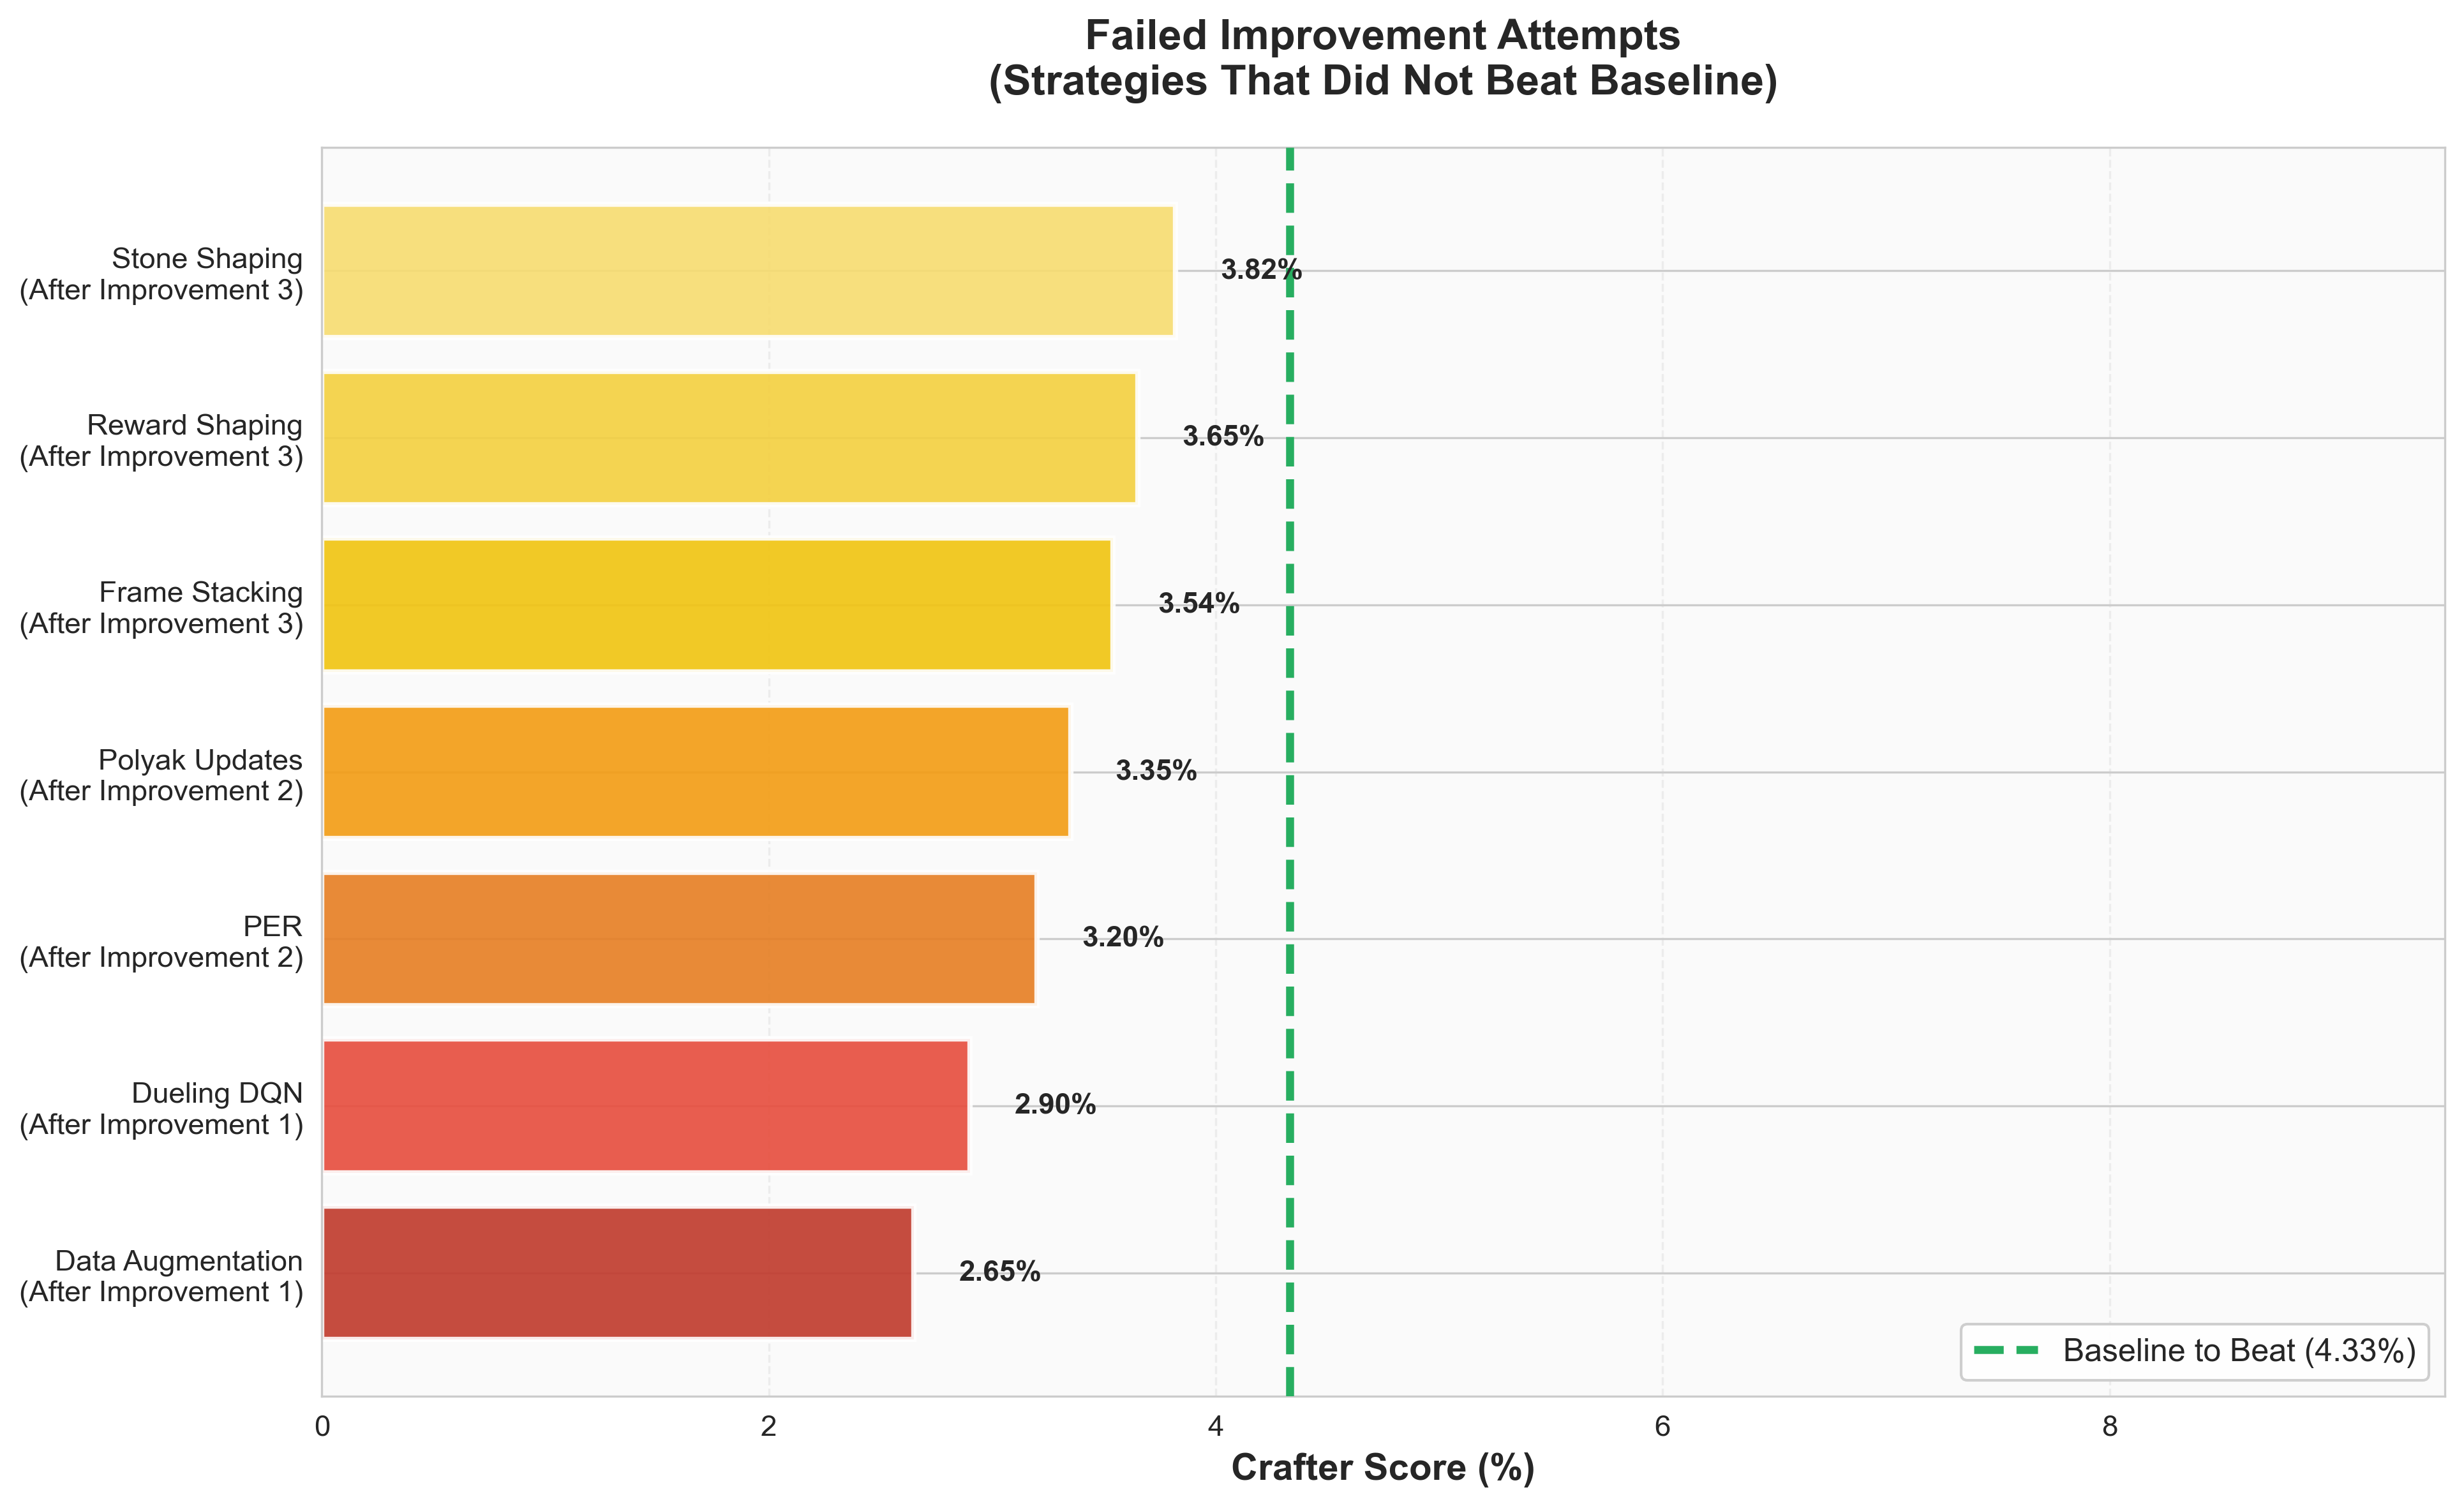
\includegraphics[width=0.48\textwidth]{fig_d4_failed_attempts.png}
\caption{DQN improvements that did not beat our then-best checkpoint (dashed line). Each bar is a full 1M-step run evaluated over 500 deterministic episodes. Augmentation, Dueling, PER, Polyak, FrameStack, and heavy shaping all underperformed in our budget.}
\label{fig:dqn_failed}
\end{figure}


\subsection{Summary of DQN Results}
Improvements form a coherent chain: better credit assignment ($n$-step) $\rightarrow$ efficient interaction (masking) $\rightarrow$ loop avoidance (random-valid) $\rightarrow$ gentle early exploration (ICM-lite) $\rightarrow$ sustained exploration (NoisyNets). The final agent reaches \textbf{5.93\%} with longer survival and higher tool/stone rates while keeping foundations stable. Coal remains the key bottleneck for DQN, indicating exploration is broader but still not reliably task-directed at that depth. \smallskip
\noindent\textit{Brief compliance note.} Each improvement is a substantive change to either the learning target (\mbox{$n$-step} returns), the policy/model (NoisyNets), or the MDP interface (action masking, random-valid fallback, train-only curiosity), rather than hyperparameter tuning.


\begin{figure}[h!]
\centering
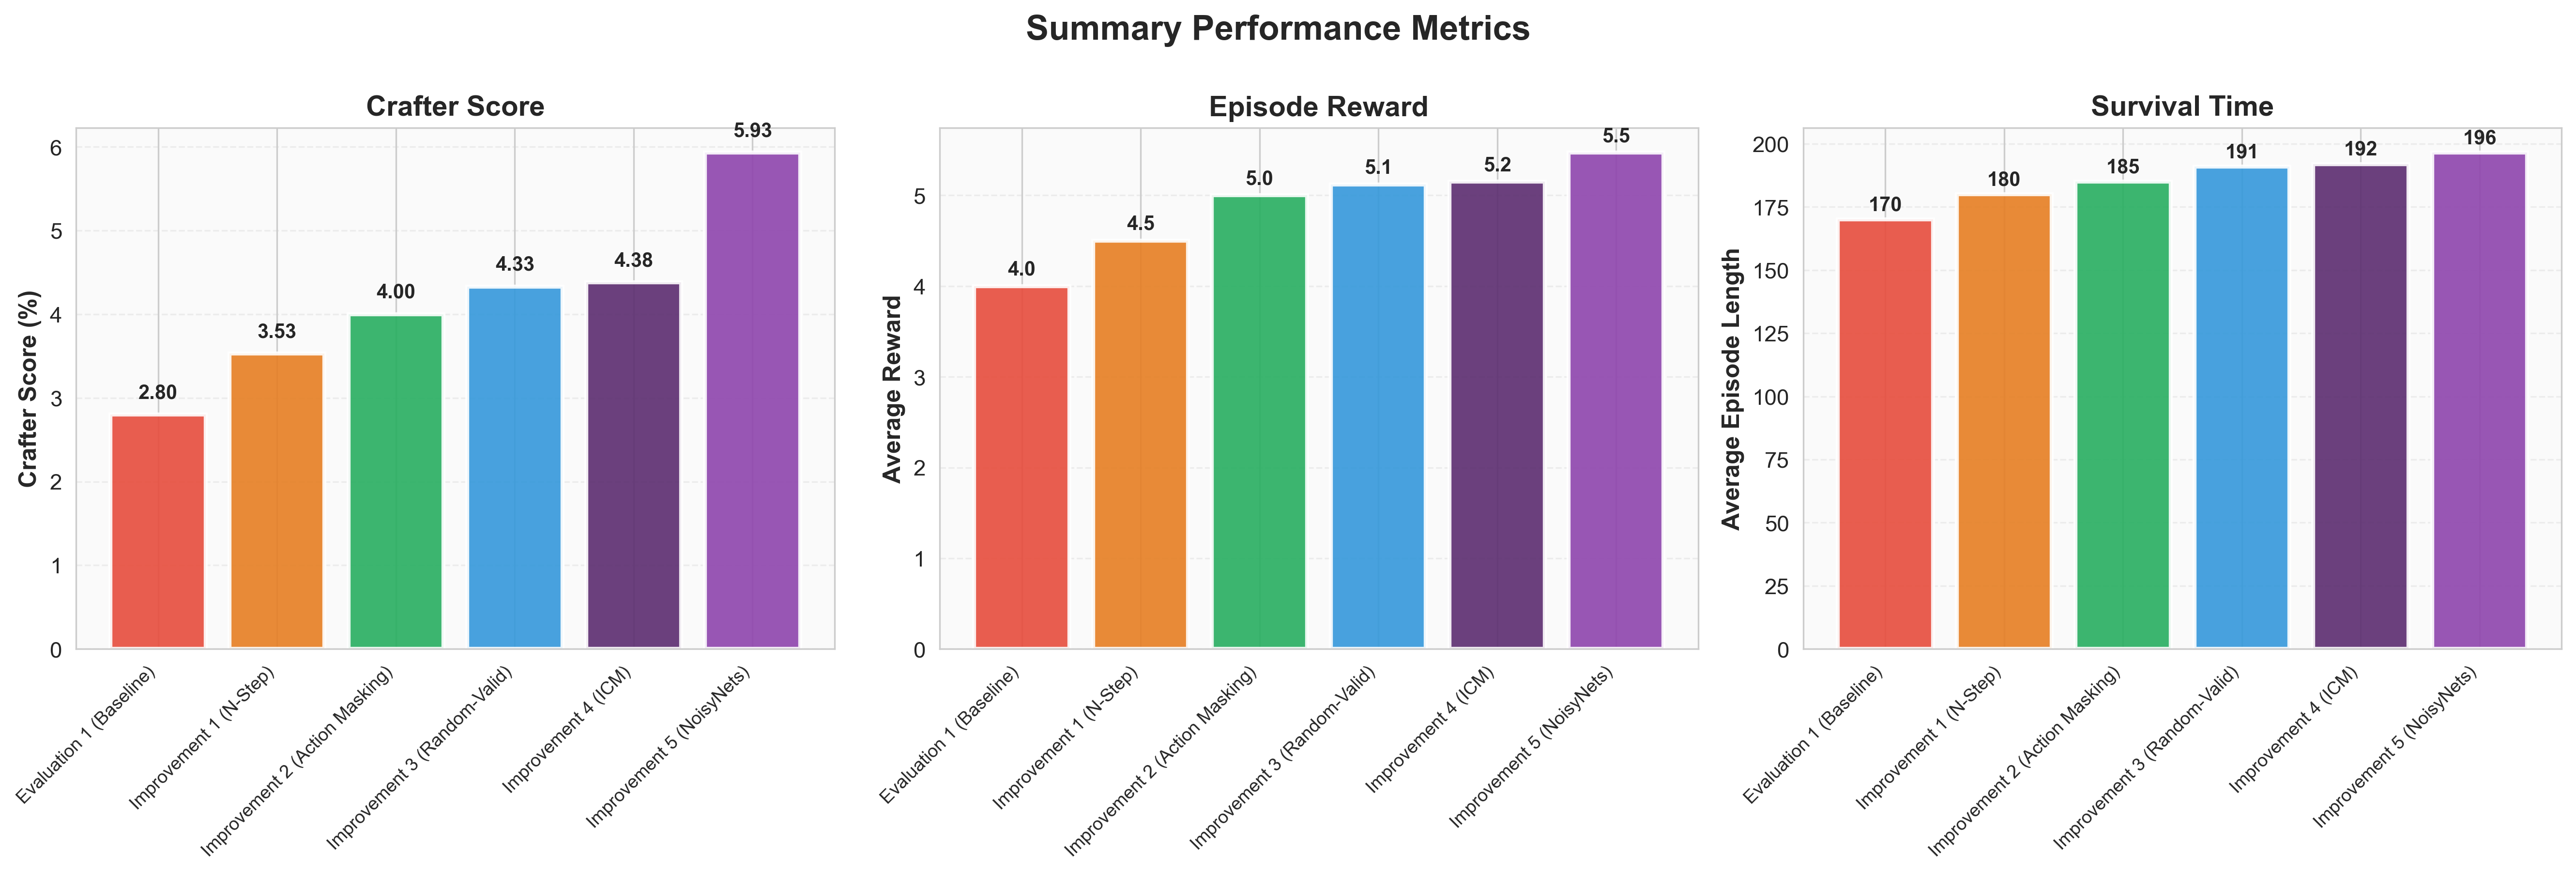
\includegraphics[width=0.48\textwidth]{fig_d3_summary_metrics.png}
\caption{Crafter Score, average reward and survival (mean over 500 episodes). Each successful step improves one or more metrics; NoisyNets yields the largest jump.}
\label{fig:dqn_summary}
\end{figure}

\begin{figure}[h!]
\centering
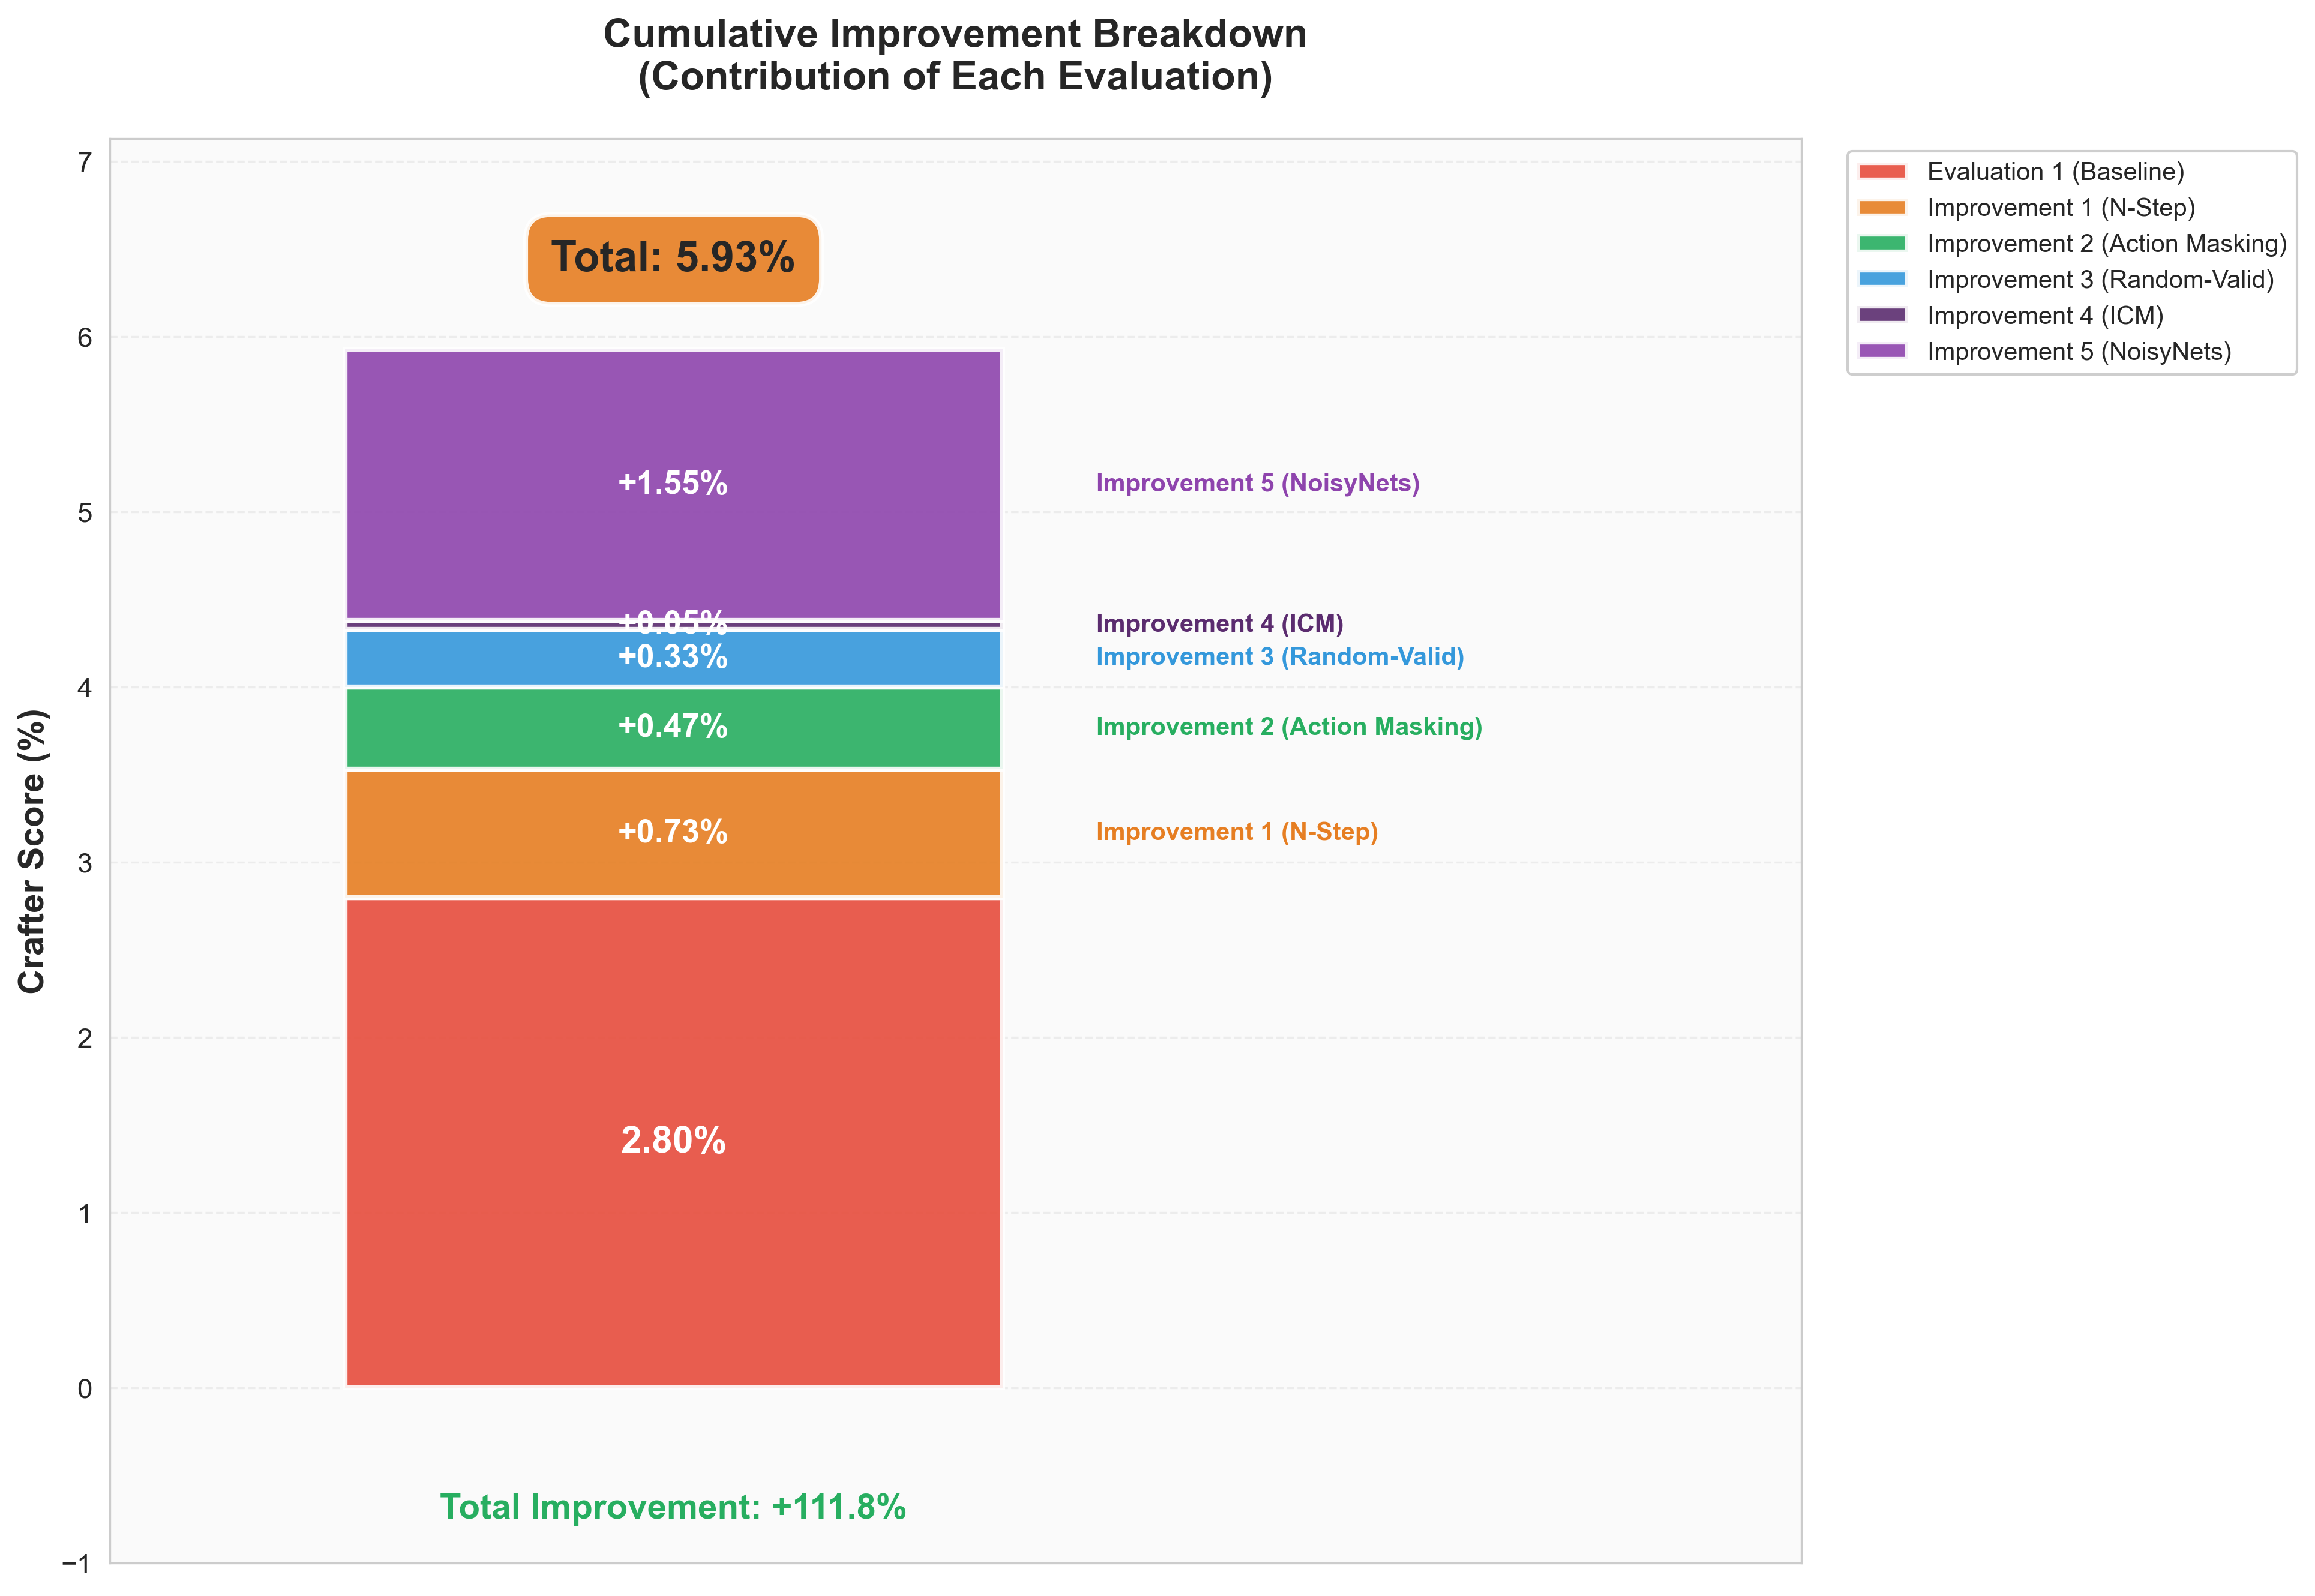
\includegraphics[width=0.48\textwidth]{fig_d5_cumulative_improvement.png}
\caption{Cumulative improvement breakdown from 2.80\% to 5.93\%. Approx.\ contributions: +0.73 (Imp.~1), +0.47 (Imp.~2), +0.33 (Imp.~3), +0.05 (Imp.~4), +1.55 (Imp.~5).}
\label{fig:dqn_breakdown}
\end{figure}


\section{Comparing PPO and DQN}

\subsection{Final Scores}

Table \ref{tab:results} shows our final results:

\begin{table}[h]
\centering
\caption{Final Results Comparison}
\label{tab:results}
\begin{tabular}{lcc}
\toprule
\textbf{Metric} & \textbf{PPO} & \textbf{DQN} \\
\midrule
Final Score & \textbf{8.61\%} & 5.93\% \\
Improvement & \textbf{+69.5\%} (5.08$\rightarrow$8.61) & +111.8\% (2.80$\rightarrow$5.93) \\
Training Time & \textbf{2.5 hours} & 5--6 hours (1M steps, CUDA) \\
Wood Pickaxe & \textbf{58\%} & 21\% \\
Wood Sword & \textbf{61\%} & 27\% \\
Coal (rare) & \textbf{2\%} & 0\% \footnotesize{(hit 0.20\% in Imp.~4)} \normalsize \\
Stone & 17\% & \textbf{2.4\%} \\
Zombie Combat & 61\% & \textbf{55.6\%} \\
\bottomrule
\end{tabular}
\end{table}

\subsection{Exploration Strategies}

The biggest difference between the algorithms was exploration:

\textbf{PPO used ICM curiosity-driven exploration:}
\begin{itemize}
    \item Gave dense intrinsic rewards for novel state transitions
    \item Successfully found rare achievements (coal 2\%, skeleton 2\%)
    \item Balanced exploration-exploitation with $\beta=0.15$ (15\% curiosity weight)
    \item Required careful tuning to avoid curiosity traps (failed at $\beta=0.3$)
\end{itemize}

\textbf{DQN used NoisyNets + action masking:}
\begin{itemize}
    \item Parameter noise in Q-network for sustained exploration
    \item Inventory-aware action masking to eliminate invalid actions
    \item Random-valid fallback prevented NOOP loops
    \item Conservative ICM-lite bonus (train-only, capped at 10\% of median return)
    \item Struggled with very rare achievements (coal 0\% in final, briefly 0.20\%)
\end{itemize}

\subsection{What We Learned}

\textbf{About sparse rewards:} Standard exploration methods struggle. Curiosity-driven exploration helped PPO find rare achievements that would never be discovered by random chance.

\textbf{About hyperparameters:} Literature values worked much better than our initial guesses. It's worth checking published implementations for starting points.

\textbf{About experimentation:} We tried 11+ different strategies. Many failed, but failures taught us important lessons about what doesn't work.

\textbf{About training:} Training metrics during learning don't always predict final performance. Always evaluate the final model separately.

\subsection{Which Algorithm Worked Better?}

\textbf{PPO achieved a higher final score (8.61\% vs 5.93\%)} and demonstrated superior performance on Crafter's sparse-reward environment.

\textbf{Why PPO performed better:}
\begin{itemize}
    \item \textbf{Stronger exploration:} ICM curiosity provided consistent intrinsic rewards throughout training, helping discover rare achievements (coal, skeleton) that DQN never reliably found
    \item \textbf{Policy representation:} PPO's stochastic policy naturally maintains exploration while DQN's $\epsilon$-greedy/NoisyNets struggled to balance exploration-exploitation at long horizons
    \item \textbf{Training efficiency:} PPO converged faster (2.5 hours vs 5-6 hours) with simpler implementation
    \item \textbf{Breadth of achievements:} PPO achieved higher rates across most categories (wood tools 58-61\% vs 21-27\%, coal 2\% vs 0\%)
\end{itemize}

\textbf{Trade-offs and DQN advantages:}
\begin{itemize}
    \item \textbf{Relative improvement:} DQN showed larger relative gains (+111.8\% vs +69.5\%) from a weaker baseline
    \item \textbf{Sample efficiency potential:} DQN's experience replay allows reusing samples, though this didn't overcome exploration limitations in practice
    \item \textbf{Action masking innovation:} DQN's inventory-aware masking (valid action set) was clever but couldn't fully compensate for weaker exploration
    \item \textbf{Systematic debugging:} DQN's approach showed rigorous analysis of failure modes (NOOP loops, invalid actions)
\end{itemize}

\textbf{Key insight:} For Crafter's compositional, sparse-reward structure, \emph{exploration quality matters more than sample efficiency}. PPO's curiosity-driven approach discovered the necessary action sequences, while DQN's masking made interactions efficient but couldn't guide discovery of rare, multi-step achievements.

\subsection{Project Limitations}

\begin{itemize}
    \item Only tested on one environment (Crafter)
    \item Limited compute (~30-40 hours total)
    \item Manual hyperparameter tuning
    \item Could not test more advanced methods (hierarchical RL, etc.)
\end{itemize}

\subsection{If We Had More Time}

\begin{itemize}
    \item Test on other sparse-reward environments
    \item Try combining best parts of both algorithms
    \item Automated hyperparameter search
    \item Test hierarchical approaches for multi-step tasks
\end{itemize}

\section{Conclusion}

This project taught us how to implement and improve reinforcement learning algorithms from scratch. Starting from weak baselines, we systematically tested improvements and learned what works in sparse-reward environments.

\textbf{PPO achieved the best overall performance (8.61\%, +69.5\% improvement)} through better hyperparameters (lr=5e-4, entropy=0.001), ICM curiosity-driven exploration ($\beta$=0.15), and increased network capacity (1024 hidden units). The ICM module proved critical for discovering rare achievements like coal (2\%) and skeletons (2\%) that require long action sequences.

\textbf{DQN achieved 5.93\% (+111.8\% improvement from 2.80\% baseline)} through a systematic sequence of targeted changes: $n$-step returns ($n$=3), inventory-aware action masking with random-valid fallback, train-only ICM-lite curiosity, and NoisyNets with hard target updates. Each change addressed a measured weakness (credit assignment, wasted actions, NOOP loops, sustained exploration). However, DQN struggled with very rare achievements (coal 0\% final) due to exploration limitations.

\textbf{PPO proved more effective for Crafter} because curiosity-driven exploration fundamentally outperformed action masking for rare achievement discovery in compositional tasks with sparse rewards.

Key lessons:
\begin{itemize}
    \item \textbf{Exploration quality > sample efficiency:} ICM curiosity discovered rare achievements that $\epsilon$-greedy and NoisyNets missed
    \item \textbf{Curiosity needs balance:} Too much ($\beta$=0.3) creates curiosity traps; too little misses rare states
    \item \textbf{Literature values matter:} Standard hyperparameters outperformed initial guesses significantly
    \item \textbf{Document failures:} 7 PPO failures (RND, high entropy, extended training) taught us what doesn't work
    \item \textbf{Training metrics $\neq$ eval performance:} PPO's best model (8.61\% eval) had lower training reward (5.14) than a worse model
\end{itemize}

Code available at: \textit{[GitHub link]}

\begin{thebibliography}{9}

\bibitem{schulman2017}
J. Schulman et al., ``Proximal policy optimization algorithms,'' 2017.

\bibitem{mnih2015}
V. Mnih et al., ``Human-level control through deep reinforcement learning,'' Nature, 2015.

\bibitem{hafner2021}
D. Hafner, ``Benchmarking the spectrum of agent capabilities,'' 2021.

\bibitem{pathak2017}
D. Pathak et al., ``Curiosity-driven exploration by self-supervised prediction,'' 2017.

\bibitem{burda2019}
Y. Burda et al., ``Exploration by random network distillation,'' 2019.

\bibitem{schulman2016}
J. Schulman et al., ``High-dimensional continuous control using GAE,'' 2016.

\bibitem{vanhasselt2016}
H. van Hasselt, A. Guez, and D. Silver, ``Deep reinforcement learning with double Q-learning,'' AAAI, 2016.

\bibitem{hessel2018}
M. Hessel et al., ``Rainbow: Combining improvements in deep reinforcement learning,'' AAAI, 2018.

\bibitem{wang2016dueling}
Z. Wang et al., ``Dueling Network Architectures for Deep Reinforcement Learning,'' ICML, 2016.

\bibitem{fortunato2018}
M. Fortunato et al., ``Noisy networks for exploration,'' ICLR, 2018.

\bibitem{schaul2016}
T. Schaul, J. Quan, I. Antonoglou, and D. Silver, ``Prioritized experience replay,'' ICLR, 2016.

\bibitem{lillicrap2016}
T. P. Lillicrap et al., ``Continuous control with deep reinforcement learning,'' ICLR, 2016. % soft/Polyak targets

\bibitem{suttonbarto2018}
R. S. Sutton and A. G. Barto, \textit{Reinforcement Learning: An Introduction}, 2nd ed., 2018.


\end{thebibliography}

\end{document}